\chapter[A$\beta$42]{Molecular Mechanism of A$\beta$42 fibril inhibition by inositol}

% Some notes
% I found these pretty neat ref articles on sciencedirect
% http://www.sciencedirect.com.myaccess.library.utoronto.ca/science/article/pii/B9780444519672001550
% http://www.sciencedirect.com.myaccess.library.utoronto.ca/science/article/pii/B9780444519672000581
% http://www.sciencedirect.com.myaccess.library.utoronto.ca/science/article/pii/B9780444519672000313
% http://www.sciencedirect.com.myaccess.library.utoronto.ca/science/article/pii/B0080437486011592

	
\section{Summary}
Alzheimer's disease (AD) is a severe neurodegenerative disease with no cure. Currently, one method of targeting the underlying disease is to prevent or reverse the amyloid formation of A$\beta$42, a key pathological hallmark of AD. A small-molecule novel drug candidate, Scyllo-inositol, is a polyol small-molecule that exhibits stereochemistry dependent inhibition of the formation of fibrils in vitro.  Furthermore, recently completed phase II clinical trials demonstrated that scyllo-inositol achieved target drug levels in the cerebral spinal fluid (CSF) of AD patients, a main challenge for AD drug candidates to overcome.

Despite its promise as a therapeutic for AD, the mechanism of action of scyllo-inositol at the molecular level is currently not understood.  We perform extensive atomistic molecular dynamics simulations of scyllo-inositol and its inactive stereoisomer, chiro-inositol, glucose, and the osmolyte protein stabilizer, glycerol, with the full length A$\beta$42 protofibril.  From our simulations, we characterize the stereochemistry-dependent binding modes of these three cosolutes on the structure and aggregation of A$\beta$42 protofibrils.  Our results provide molecular insight for the rational design of small-molecule inhibitors of A$\beta$42 and other amyloid-based diseases.

  \textbf{Keywords}:
	amyloid computational
	amyloid inhibition
	small molecule amyloid inhibition
	amyloid disaggregation
	inositol
	surface binding
	weak interactions
	carbohydrate like interactions

\section{Introduction}
\abetafortytwo\ is the pathological hallmark of Alzheimer's Disease (AD) and forms the largest proteinaeous component of plaques in the brain of AD patients. \abeta\ peptides are produced from the cleavage of amyloid precursor protein (APP) in isoforms with lengths of 33 to 42 residues. Although A$\beta$42 and A$\beta$40 peptides differ in length only by two residues, \abetafortytwo\ is found to display significantly higher aggregation propensity\cite{Jarrett:1993vm,Fukumoto:1996vi,Finder:2010jw} and cellular toxicity than \abetaforty\ peptides.\cite{ElAgnaf:2000hp,Mucke:2000uqa}
% Furthermore, they are found to form fibrils via distinct pathways.\cite{Bitan:2003ut,Sanchez:2011bj,Bitan:2003p1781}
% Rationale for studying the Abeta42 protofibril system	-- there is all this abeta40 stuff simply because its easier to work with these peptides, but then abeta42 is the actual important peptide that people should be looking at!
Multiple studies have probed the aggregation properties of both \abetaforty\ and \abetafortytwo. Fibril models of the \abetaforty\ peptide derived from solid-state NMR (SSNMR) indicate that protofilaments of \abetaforty\ contain 2 to 3 layers.\cite{Wu:2010p3553,Tycko:2010iz} By contrast, much less is known about the fibril structure of \abetafortytwo. A SSNMR model of the fibril of \abetafortytwo\ was recently proposed by Luhrs et al.\cite{luhrs} In that model, N-terminus of \abetafortytwo\ in the fibril was found to be unstructured.\cite{Ahmed:2010p5694} 
% This doesn't quite belong here.
% A previous MD simulation study based on models of these \abetafortytwo\ protofibrils in pure water suggests that residues 17 to 42 are predominantly involved in the stability of the core structure of the fibril.\cite{Masman:2009p6410}

% Small molecules are promising candidates for the treatment of AD. Many of them have been found to display anti-aggregation activity, including osmolytes.
In recent years, small molecule inhibitors of \abeta\ amyloid formation have emerged as promising candidates for the treatment of Alzheimer's disease. One such molecule is \emph{scyllo}-Inositol, a inhibitor of A$\beta$42 fibrillation.\cite{McLaurin:2006eb,McLaurin:2000bq,Fenili:2007p3978,Ma:2012jk} Inositol is a class of cyclohexylpolyols, of which eight out of nine stereoisomers are commonly found in nature. \emph{scyllo}-Inositol, with all hydroxyl groups equatorial, is the only isomer with two planar hydrophobic faces. By contrast, its diastereisomer, \emph{chiro}-inositol, with two adjacent axial hydroxyl groups, has two nonplanar hydrophobic faces. 
   
\emph{In vitro}, inositol displays stereochemistry-dependent inhibition of A$\beta$42 fibrils: \emph{scyllo}-inositol was shown to inhibit A$\beta$42 fibrillation at concentrations of 1 - 5 mM,\cite{McLaurin:2000p64} whereas \emph{chiro}-inositol is inactive below molar concentrations.\cite{Janus:2000p198} Moreover, upon incubation of monomeric A$\beta$42 with \emph{scyllo}-inositol, circular dichroism spectroscopy indicated the formation of $\beta$-sheet structure at an inositol:peptide molar ratio of 25:1.\cite{McLaurin:1998p176}  

Importantly, \emph{scyllo}-inositol was demonstrated to prevent and reverse AD-like symptoms in a transgenic mouse model of AD.\cite{McLaurin:2006p29} Phase I and II of clinical trials for \emph{scyllo}-inositol (ELN0005) in North America has been completed.\cite{Salloway:2011im,Ma:2012jk} These clinical trials have demonstrated that inositol possesses positive CNS bioavailability and favorable \emph{in vivo} toxicity profile, both of which are rare and essential properties of putative AD drug candidates. Although clinical trials have successfully demonstrated the safety and tolerance profile of inositol, it is likely that further chemical modification is required to improve the efficacy of inositol as a AD therapeutic.  Understanding the molecular basis of the effect of inositol stereoisomers on A$\beta$42 will provide insight into modifications to improve the efficacy of inositol.
%Currently, although inositol stereoisomers have been proposed to inhibit amyloid formation by directly interacting with either monomers or non-fibrillar aggregates to ``cap off'' fibril growth,\cite{Janus:2000p198}
Currently, the molecular basis of the effect of \emph{scyllo}-inositol and its stereoisomers on A$\beta$42 amyloid formation is not known.
% \cite{Nikolic:2011p185,Rauscher:2006p43,Li:2012p853,Rauscher:2010p5682,Sgourakis:2011hy,Wang:2005do,Cino:2011ff}

% Don't need this -- Molecular dynamics (MD) simulations are well-suited for studies of disordered proteins and can provide atomic-level insight into the mechanism of inhibition of peptide self-aggregation by small molecules. MD simulations were previously employed to examine the binding mechanism of other small-molecule inhibitors such as polyphenols,\cite{Lemkul:2010p23,Wang:2010p204} non-steroidal anti-inflammatory drugs,\cite{Raman:2009p47,Takeda:2010p34} and the well-known amyloid dye thioflavin T\cite{Wu:2008ds,Wu:2011fd} to monomers and/or fibrillar forms of A$\beta$.\cite{Liu:2009p213}

In two previous studies (Chapters 3 and 4), we have successively examined the binding mechanism of scyllo- and chiro-inositol with peptide and aggregate states of model amyloid-forming peptides\cite{Li:2012} and A$\beta$(16-22).\cite{Li:2013}
In the study with model peptides, weak and stereochemistry independent binding of inositol with the peptidic backbone was found, with binding constants in the range of 0.1 - 1 M, indicating that inositol is unlikely to inhibit amyloid formation by binding the peptidic backbone alone (see Chapter 2). In that study, inositol was found to preferentially bind to the surface of $\beta$-sheet oligomers, but only weakly to those of disordered or monomeric forms, suggesting that the protofibril is the likely binding partner of inositol.

In the study with KLVFFAE, inositol was found to adopt cooperative, high avidity binding modes with $\beta$-oligomers with binding constants commensurate with the \emph{in vitro} inhibitory concentrations.  Taken together, results from our previous studies indicate that inositol is likely to disrupt amyloid fibrillation by binding to $\beta$-sheet oligomers of A$\beta$.

% Why study with full length ABeta fibrils now - Protofibrils of Abeta(16-22) and full-length protofibrils are different in their physical surface properties.
In this study, we examine the binding of inositol stereoisomers, scyllo- and chiro-inositol, and osmolytes glucose and glycerol with the SSNMR model of the protofibril of full-length \abetafortytwo.   Glucose and glycerol are molecules which can act as osmolytes. Osmolytes are thought to  stabilize the folded state of proteins via the preferential exclusion mechanism.\cite{Bolen:2001im}  In recent years, these osmolytes have been found to modulate amyloid formation.\cite{Sukenik:2012dv,Sukenik:2011p8778} TMAO,\cite{Seeliger:2013cj}betaine,\cite{Natalello:2009fn} glucose,\cite{Fung:2005p2008} trehalose\cite{Nayak:2009fr} and glycerol\cite{Sukenik:2011p8778} been found to modulate amyloid formation and peptide aggregation.\cite{Liu:2005km,Sukenik:2011p8778,Fung:2005p2008} \textbf{Inhibit? or promote formation?}  The molecular basis of cosolute binding to A$\beta$42 fibrils have not been previously examined. It is informative to compare the binding of glucose and glycerol, osmolytes that are not inhibitors of amyloid aggregation, and inositol stereoisomers, a known inhibitor of A$\beta$ amyloid formation. \textbf{Missing some connective logic.} 

Here, we present results which provide insight into the structure-activity relationship of inositol in the inhibition of A$\beta$ amyloid formation, which will ultimately lead to the development of a pharmcophore for treating AD and related neurodegenerative disorders.
  
\section{Material and Methods} % (fold)
\label{sec:material_and_methods}

The pentameric solid-state NMR model of A$\beta$(17-42) from Luhrs \textit{et. al.} (PDB code: 2BEG) was taken as the starting structure in our simulations.\cite{Luhrs:2005p4900} In the PDB structure, residues 1 to 16 were truncated in the model because they were found to be disordered.\cite{Luhrs:2005p4900}  The peptides were capped by acetyl groups at the N-terminal end. The acetyl groups were modelled onto the fibril structure using the PyMol software.\cite{Anonymous:2012p58} Titratable amino acids were assigned their charged states at the physiological pH. Ten sodium ions were added to neutralize remaining charges in the system. To mimic experimental conditions, 0.15 M of salt was added. Protein and solvent were represented by the OPLS-AA/L force field\cite{Jorgensen:1996vx} and the TIP3P water model\cite{Jorgensen:1983p8768} respectively.  The  extended OPLS-AA force field for carbohydrates\cite{Damm:1997tla} was used to model inositol and glucose molecules.

MD simulations were performed in the NpT ensemble using the GROMACS simulation package version 4.0.x.\cite{Hess:2008p5353} The leapfrog Verlet integration algorithm was used with an integration timestep of 2 femtoseconds. Long-range electrostatic interactions were calculated using Particle Mesh Ewald (PME) summation with a Fourier grid spacing of 0.15 nm and a real-space cutoff of 1.3 nm.\cite{Darden:1993p8963} The short-range nonbonded van der Waals interactions were switched to zero from 1.1 nm to 1.2 nm. The temperature was controlled at 300 K using the Nose-Hoover thermostat.\cite{Nose:1984wa} Pressure was controlled by the Parrinello-Rahman barostat at 1 atm with a coupling constant of 4.0 ps.\cite{Parrinello:1981vy} The SHAKE algorithm was used to constrain covalent bonds containing hydrogens.\cite{Ryckaert:1977p9357} Center of mass (COM) rotation and translation were removed at every step.

In all simulations, a cubic box geometry was used with periodic boundary conditions. Prior to data collection, 500 steps of energy minimization using the conjugate gradient algorithm was first performed.  Simulation systems were equilibrated using a two-step procedure.  First, a 200 ps equilibration was conducted in the NVT ensemble to further relax the initial configuration of the system.  Next, equilibration in the NpT ensemble (with isotropic pressure coupling) was conducted for 2 ns to relax the solvent around the protein.

In total, a set of ten 0.250 $\mu$s simulations of the protofibril of \abetafortytwo\ were performed,  successively, in pure water and in the presence of scyllo-inositol, chiro-inositol, glycerol and glucose. The ligands were present at either a ligand:peptide molar ratio of  15:5 or 64:5, yielding a total sampling time of 12.5 $\mu$s. See Table XXX for a listing of these simulations.

\subsection{Analysis Protocol}
The GROMACS analysis utilites g\_rmsd and g\_rmsf were used to calculate the root mean square deviation and root mean squared fluctuation of the fibril backbone, respectively.  Spatial probability density of bound inositol was calculated using the volmap tool implemented in the Visual Molecular Dynamics software package (VMD).\cite{vmd}

The number of hydrogen bonds between each pair of peptides in the protofibril were computed using g\_hbond.  The following geometry criteria used to determine a hydrogen bond:  (1) the distance between acceptor (A) and donor (D) heavy atoms is less than 0.35 nm, and (2) the angle formed by H-D-A is less than 30$\degreesymb$. Nonpolar contacts between inositol and fibril were defined by a carbon to carbon cutoff of 0.X nm. The DSSP algorithm was used to perform the secondary structure analysis of the protofibril.\cite{DSSP}

\section{Results and Discussion}

In the following sections below, we comparatively examine the binding of inositol stereoisomers, \textit{scyllo}-inositol and \textit{chiro}-inositol, glucose and glycerol (Figure~\ref{fig:ligands}) with the protofibril of A$\beta$42.

\begin{figure}[htbp]
  \centering
  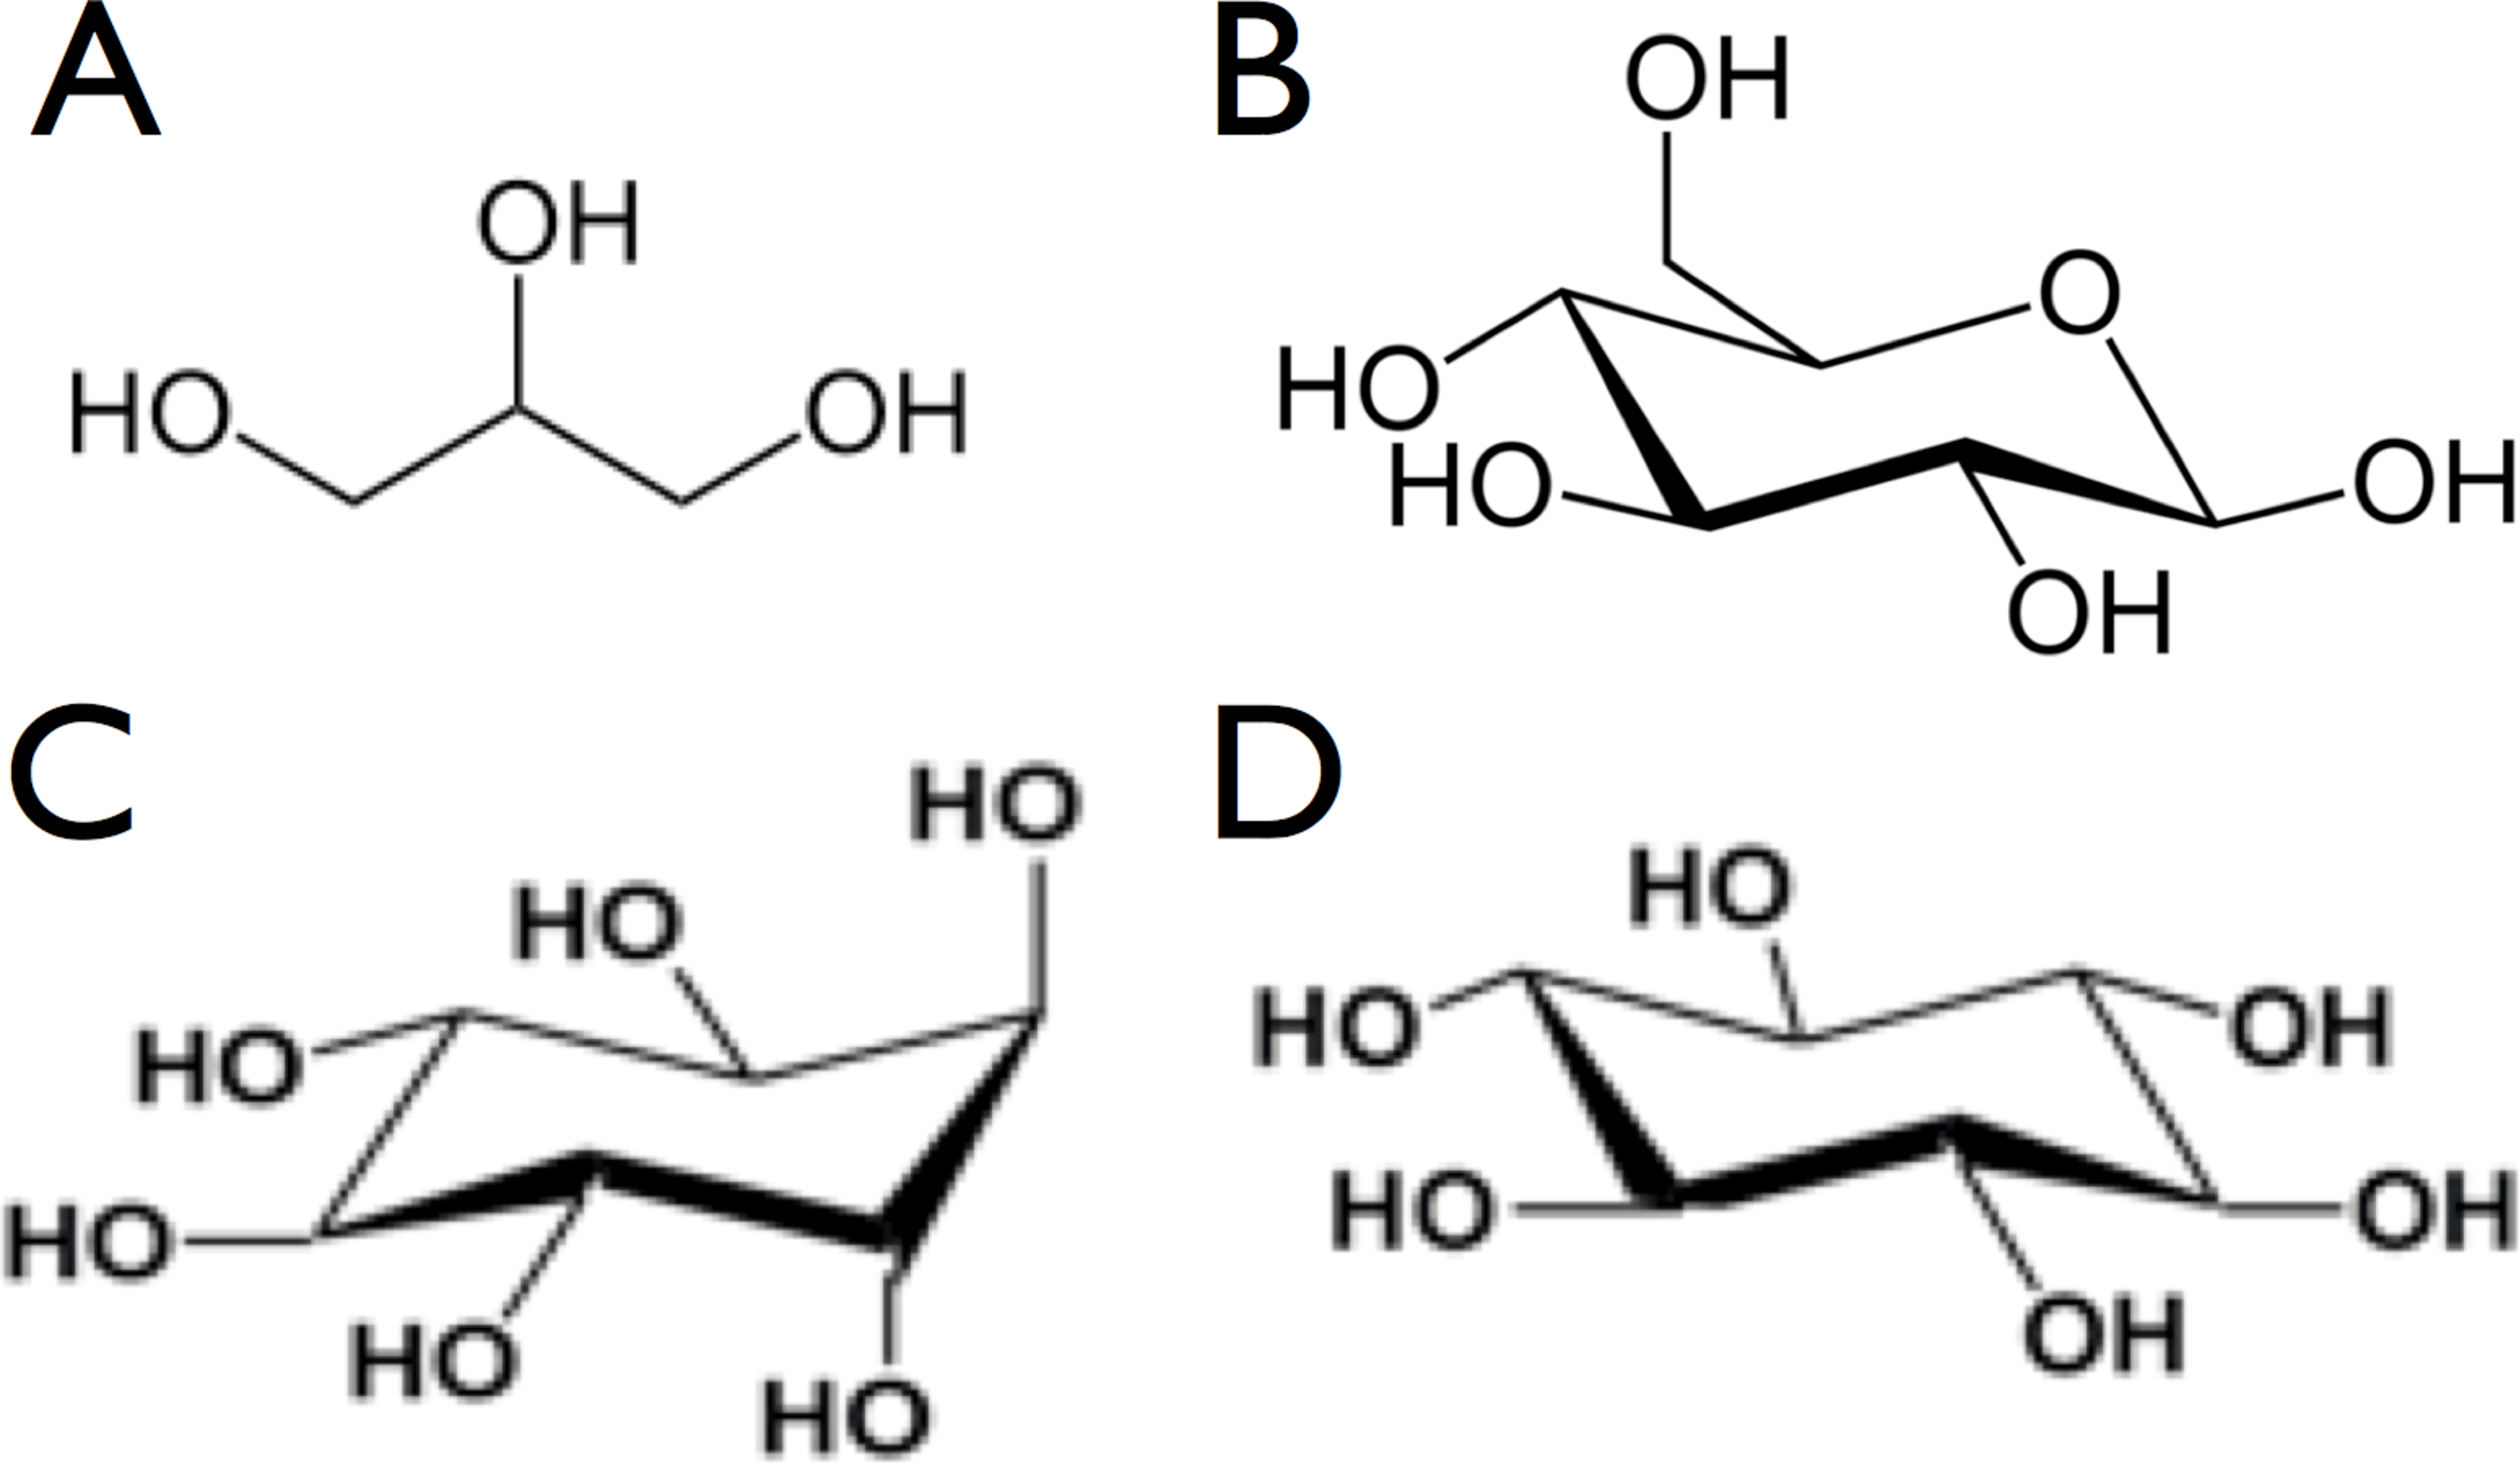
\includegraphics[width=2.5in]{figures/results3/ligands.pdf}
  \caption[Ligands]{Molecular structures of (A) glycerol, (B) glucose, (C) chiro-inositol and (D) scyllo-inositol}
  \label{fig:ligands}
\end{figure}

\subsection{Protofibrillar morphology}

We first examine the global structural properties of the fibril fragment by examining the time evolution of the RMSD and RMSF (root mean squared fluctuations) of the protofibril. In the absence and presence of the ligands (\textit{scyllo}-, \textit{chiro}-inositol, glucose and glycerol, the RMSD of the protofibril over the course of 250 ns plateaued at ~0.5 nm  (Figure~\ref{fig:protofibril_dynamics}A).  RMSF vs. t depicted in Figure~\ref{fig:protofibril_dynamics}B shows the deviation of the position of each residue from its average position. RSMF of the residues in the protofibril vary approximately between X nm and Y nm along each chain, suggesting that the protofibrillar structure is dynamic.  Both RMSD and RSMF vs. t of the protofibril were independent of the presence of ligands. Although chains at the edges of the fibril were observed to detach partially from the core of the protofibril in some of our trajectories, the $\beta$-sheet core of the protofibril stays intact throughout the simulation. The secondary structure of the protofibril was predominantly $\beta$-sheet in conformation in both the presence and absence of the ligands. Taken together, our results suggest that the fibril morphology is not affected by the presence of the ligands on the time scale of our simulations. 

\begin{figure}[htbp]
  \centering
  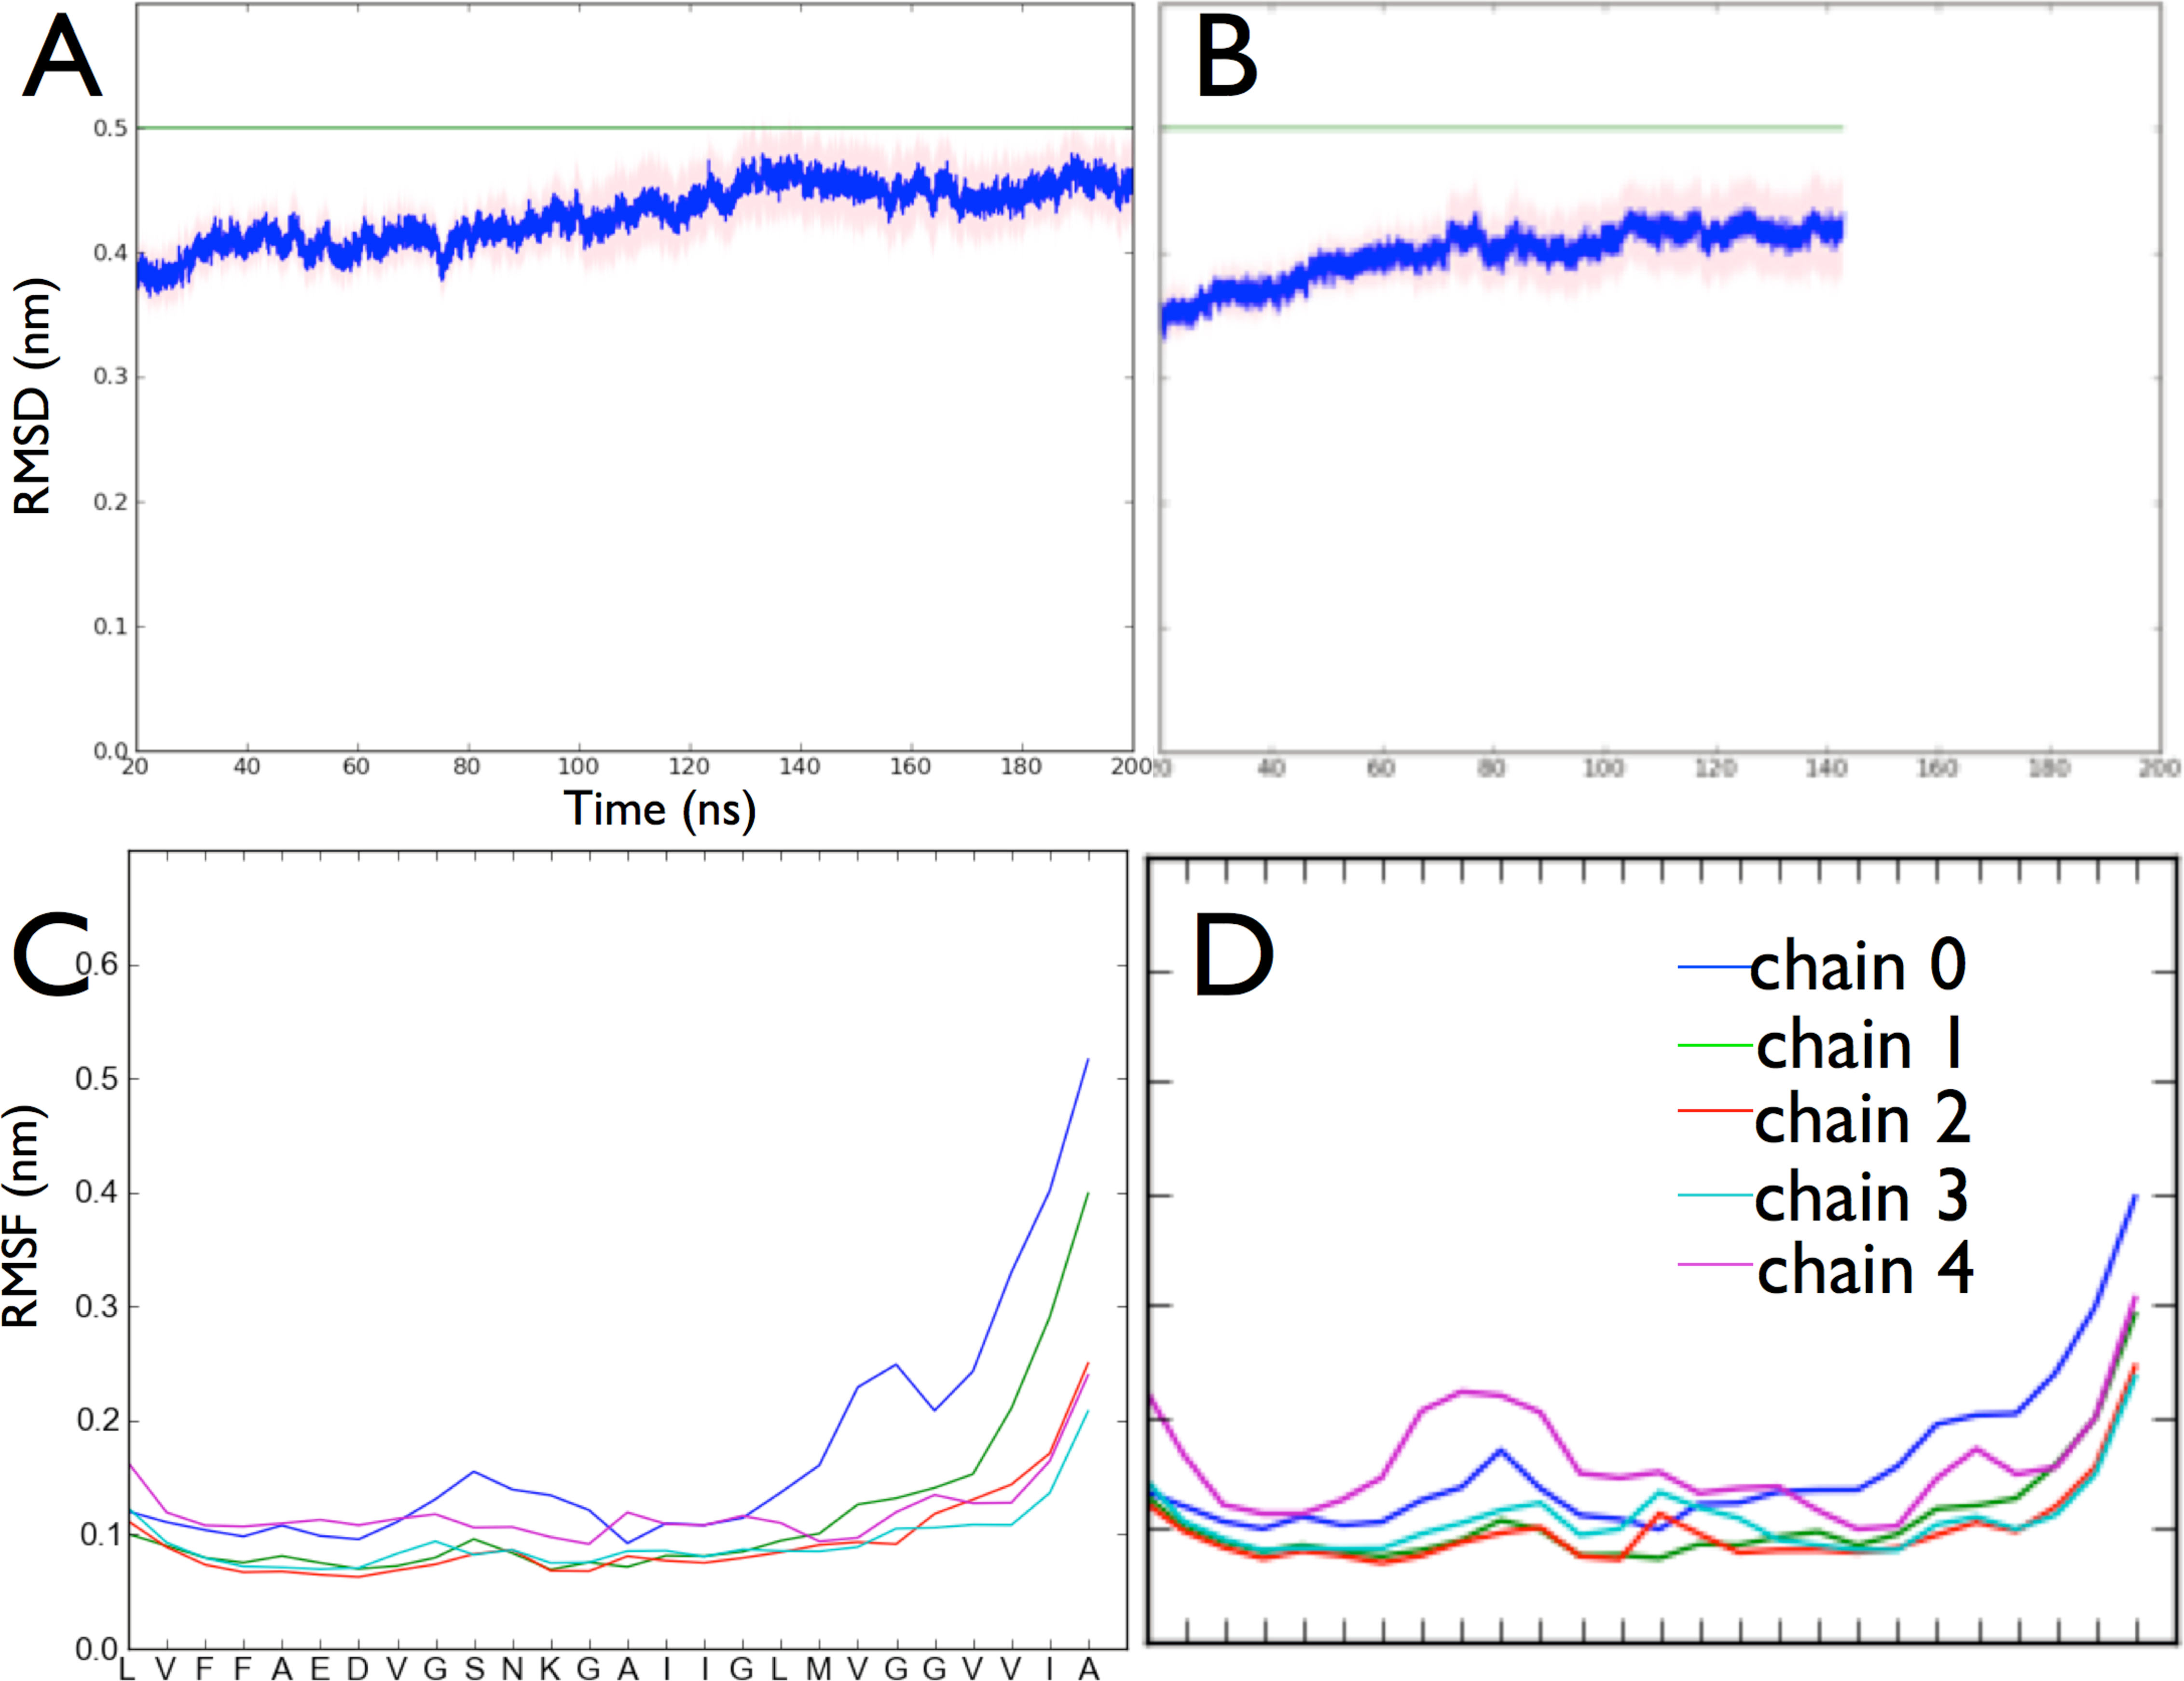
\includegraphics[width=5in]{figures/results3/protofibril_dynamics.pdf}
  \caption[RMSD and RMSF vs. time]{Fibril structure dynamics in pure water (A) and (C), and in the presence of scyllo-inositol (B) and (D).}
  \label{fig:protofibril_dynamics}
\end{figure}

\subsection{Comparison of binding modes}
% Qualitative description of the major binding modes
The protofibril presents two chemically different $\beta$-sheet faces. The $\beta$1 face contains residues in the central hydrophobic core of A$\beta$, LVFFA and possesses a negative-charged region formed by a row of solvent-exposed Glu22. In contrast, the second face of the protofibril ($\beta$2) presents a predominantly hydrophobic surface containing the residues IIGLMVGGVVIA (Figure~\ref{protofibril_dynamics}E).  

Scyllo-, chiro-inositol and glucose molecules all bound to the surface of the protofibril (Figure~\ref{fig:spatial_binding}) and were found to partitioned to four main binding sites on the protofibril: (1) $\beta$1 face, (2) $\beta$2 face,  (3) edges,  and (4) a channel-like crevice formed between the two $\beta$-sheets.

Depicted in Figure~\ref{fig:spatial_binding}, \textit{scyllo}-inositol predominantly bound to the $\beta$1 face rather than the $\beta$2 face. By contrast, both \textit{chiro}-inositol and glucose possessed significantly less density on the $\beta$1 face, and instead displayed significant binding densities on the $\beta$2 face.  
Binding contact maps indicate that binding to this face is localized to the residues Phe20 and Glu22 (Figure~\ref{fig:binding_map}).  As shown in Figure~\ref{fig:detailed_binding_modes}, all three molecules adopt binding modes to the $\beta$1 face via a combination of hydrogen bonding to Glu22 and forming nonpolar contacts with Phe20. 

In contrast to both inositol and glucose, glycerol did not possess significant binding density on either faces (Figure~\ref{fig:spatial_binding}C). Because glycerol did not bind to the solvent-exposed surface of the protofibril, in the sections below the term ligands will be used to collectively refer to scyllo-, chiro-inositol and glucose for clarity.

\begin{figure}[htbp]
  \centering
  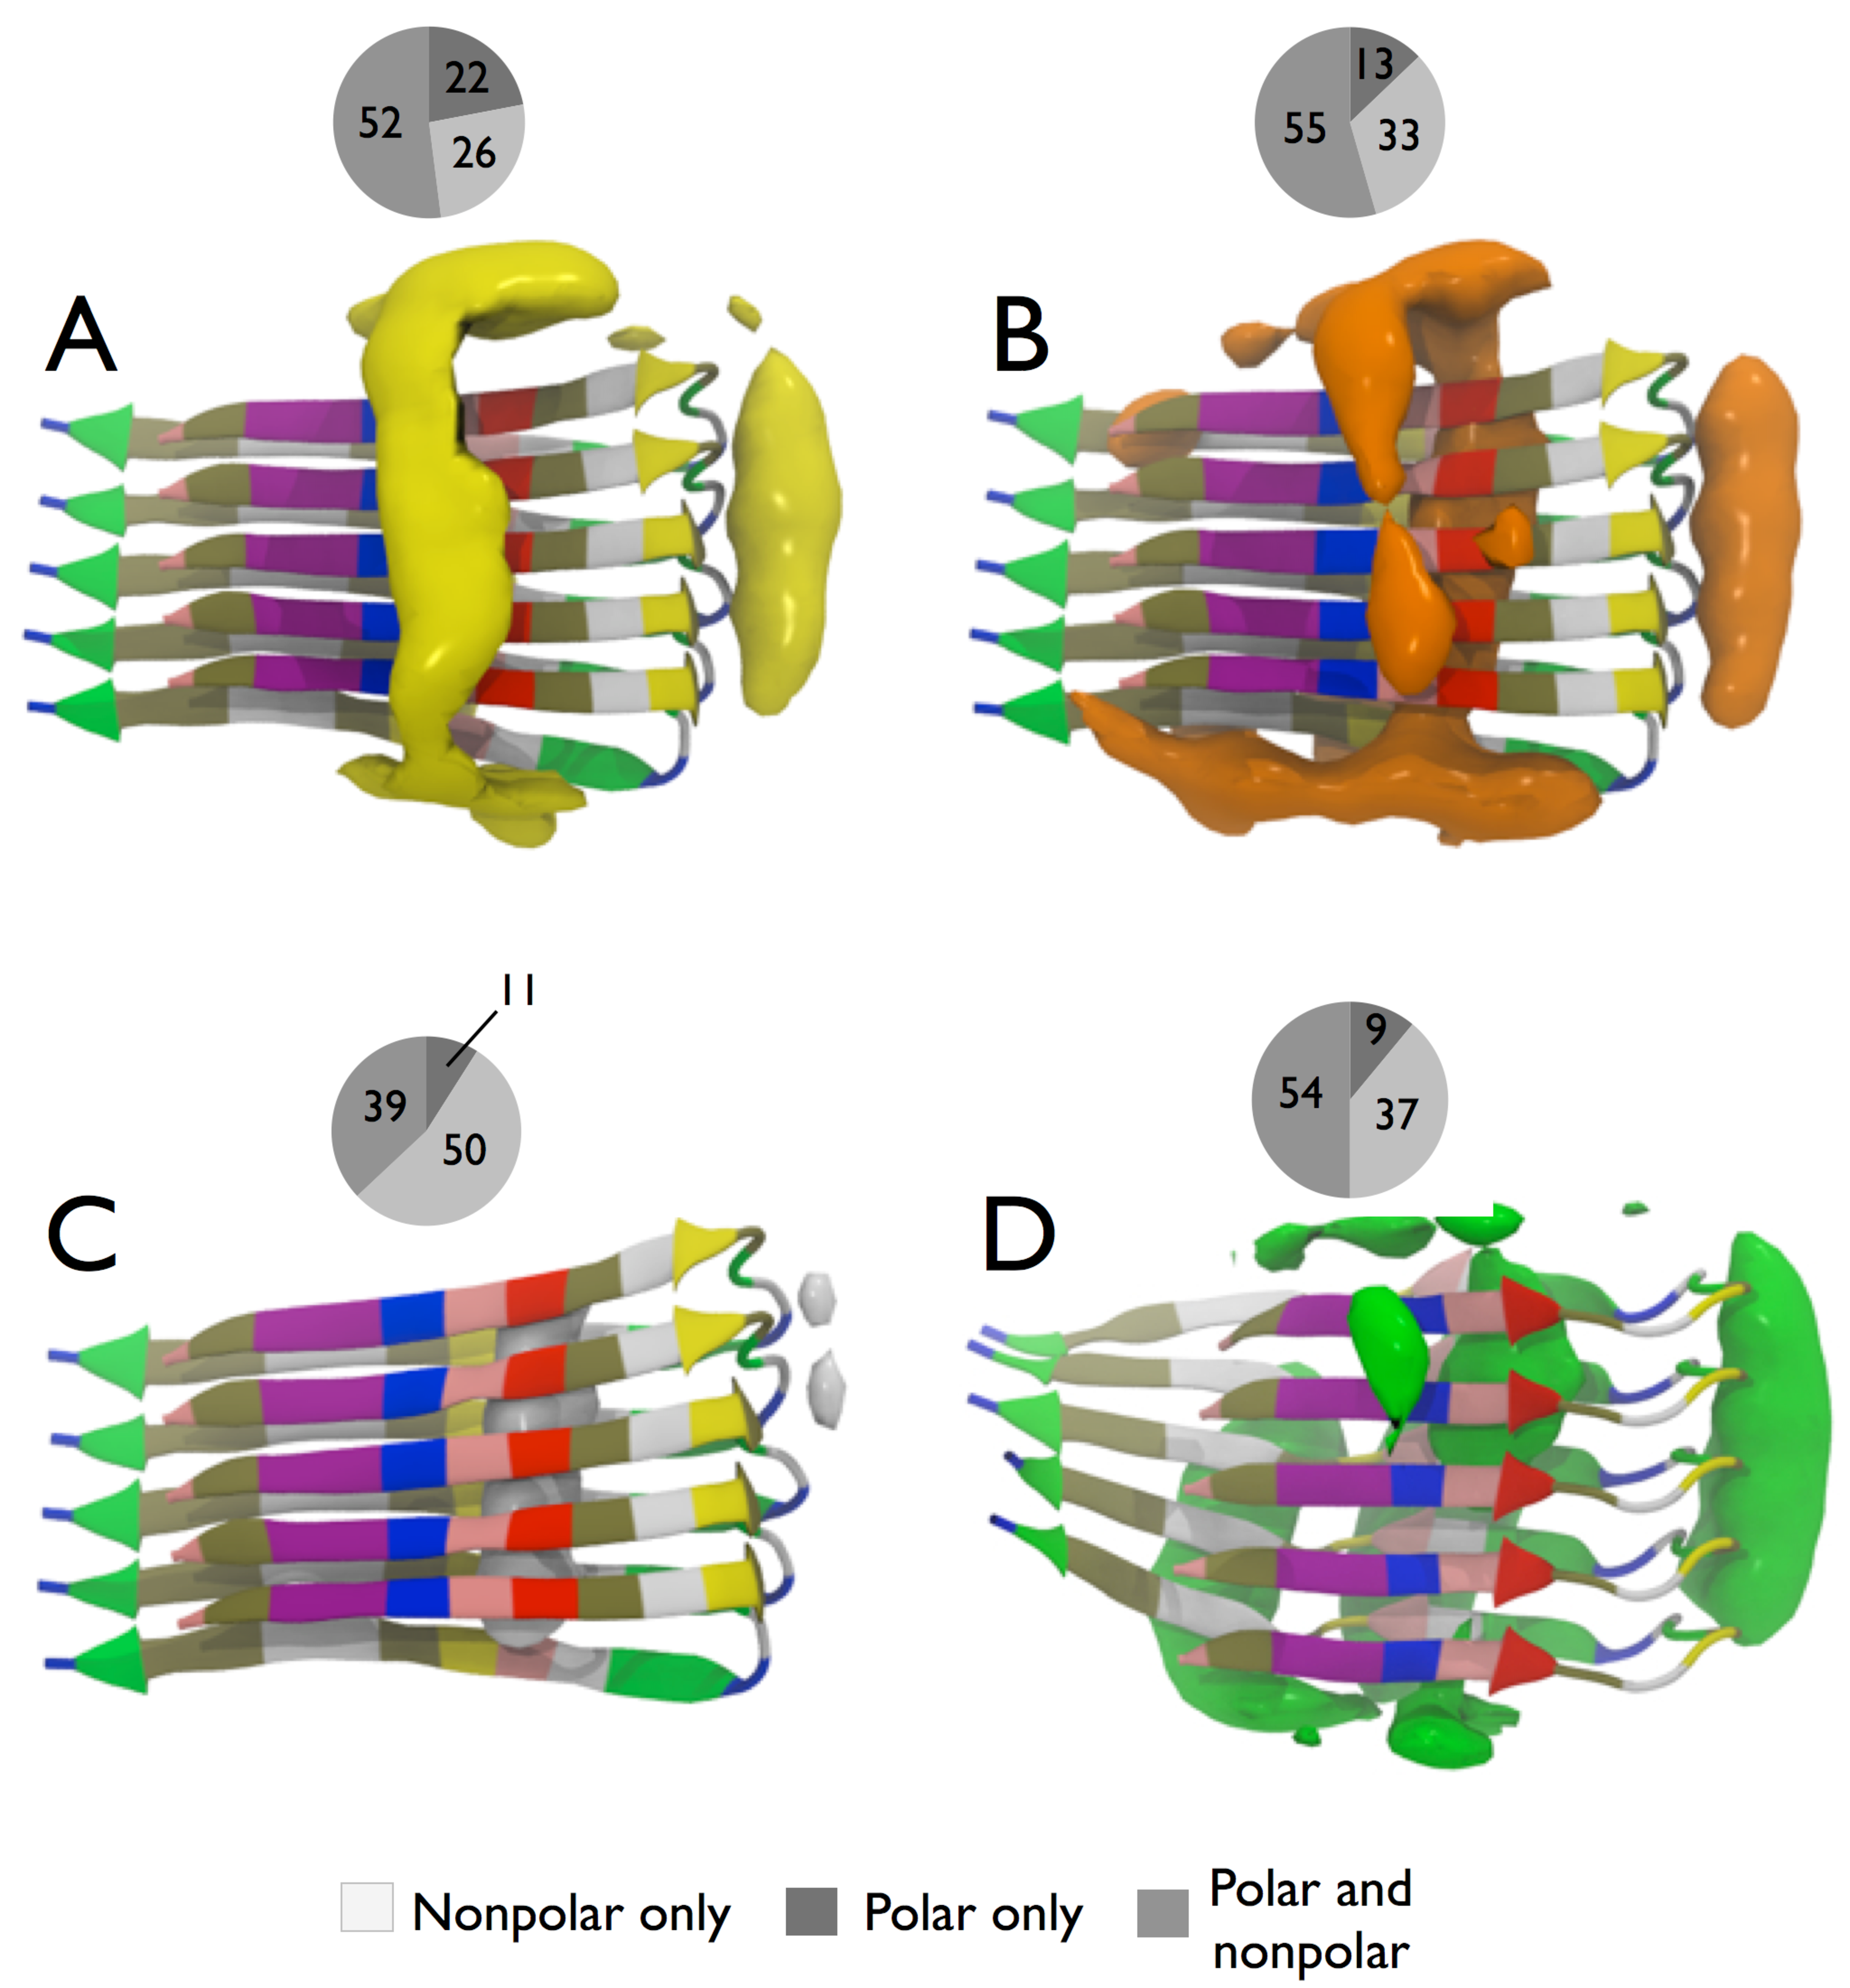
\includegraphics[width=6in]{figures/results3/binding_sdf_pie_chart.pdf}
  \caption[Spatial probability distribution of bound solutes]{Comparisons of the spatial binding probability densities and binding modes for (A) scyllo-inositol, (B) chiro-inositol, (C) glycerol and (D) glucose.}
  \label{fig:spatial_binding}
\end{figure}

A second location with significant binding density are the grooves located at the edges of the $\beta$-strands of the protofibril. Both Chiro-inositol and glucose bound non-specifically to residues along the entire edge, whereas the scyllo-inositol displayed more localized binding (Figure~\ref{fig:spatial_binding}, \ref{fig:binding_map}).
%\textbf{The ligand-protofibril contact maps shown in Figure~\ref{fig:} indicate that ...[ elaborate - which residues? Look at the contact map ].}
We speculate that binding at the edges may slow elongation or strand addition, but is unlikely to arrest growth of a protofibril into amyloid fibrils.

\begin{figure}[htbp]
  \centering
  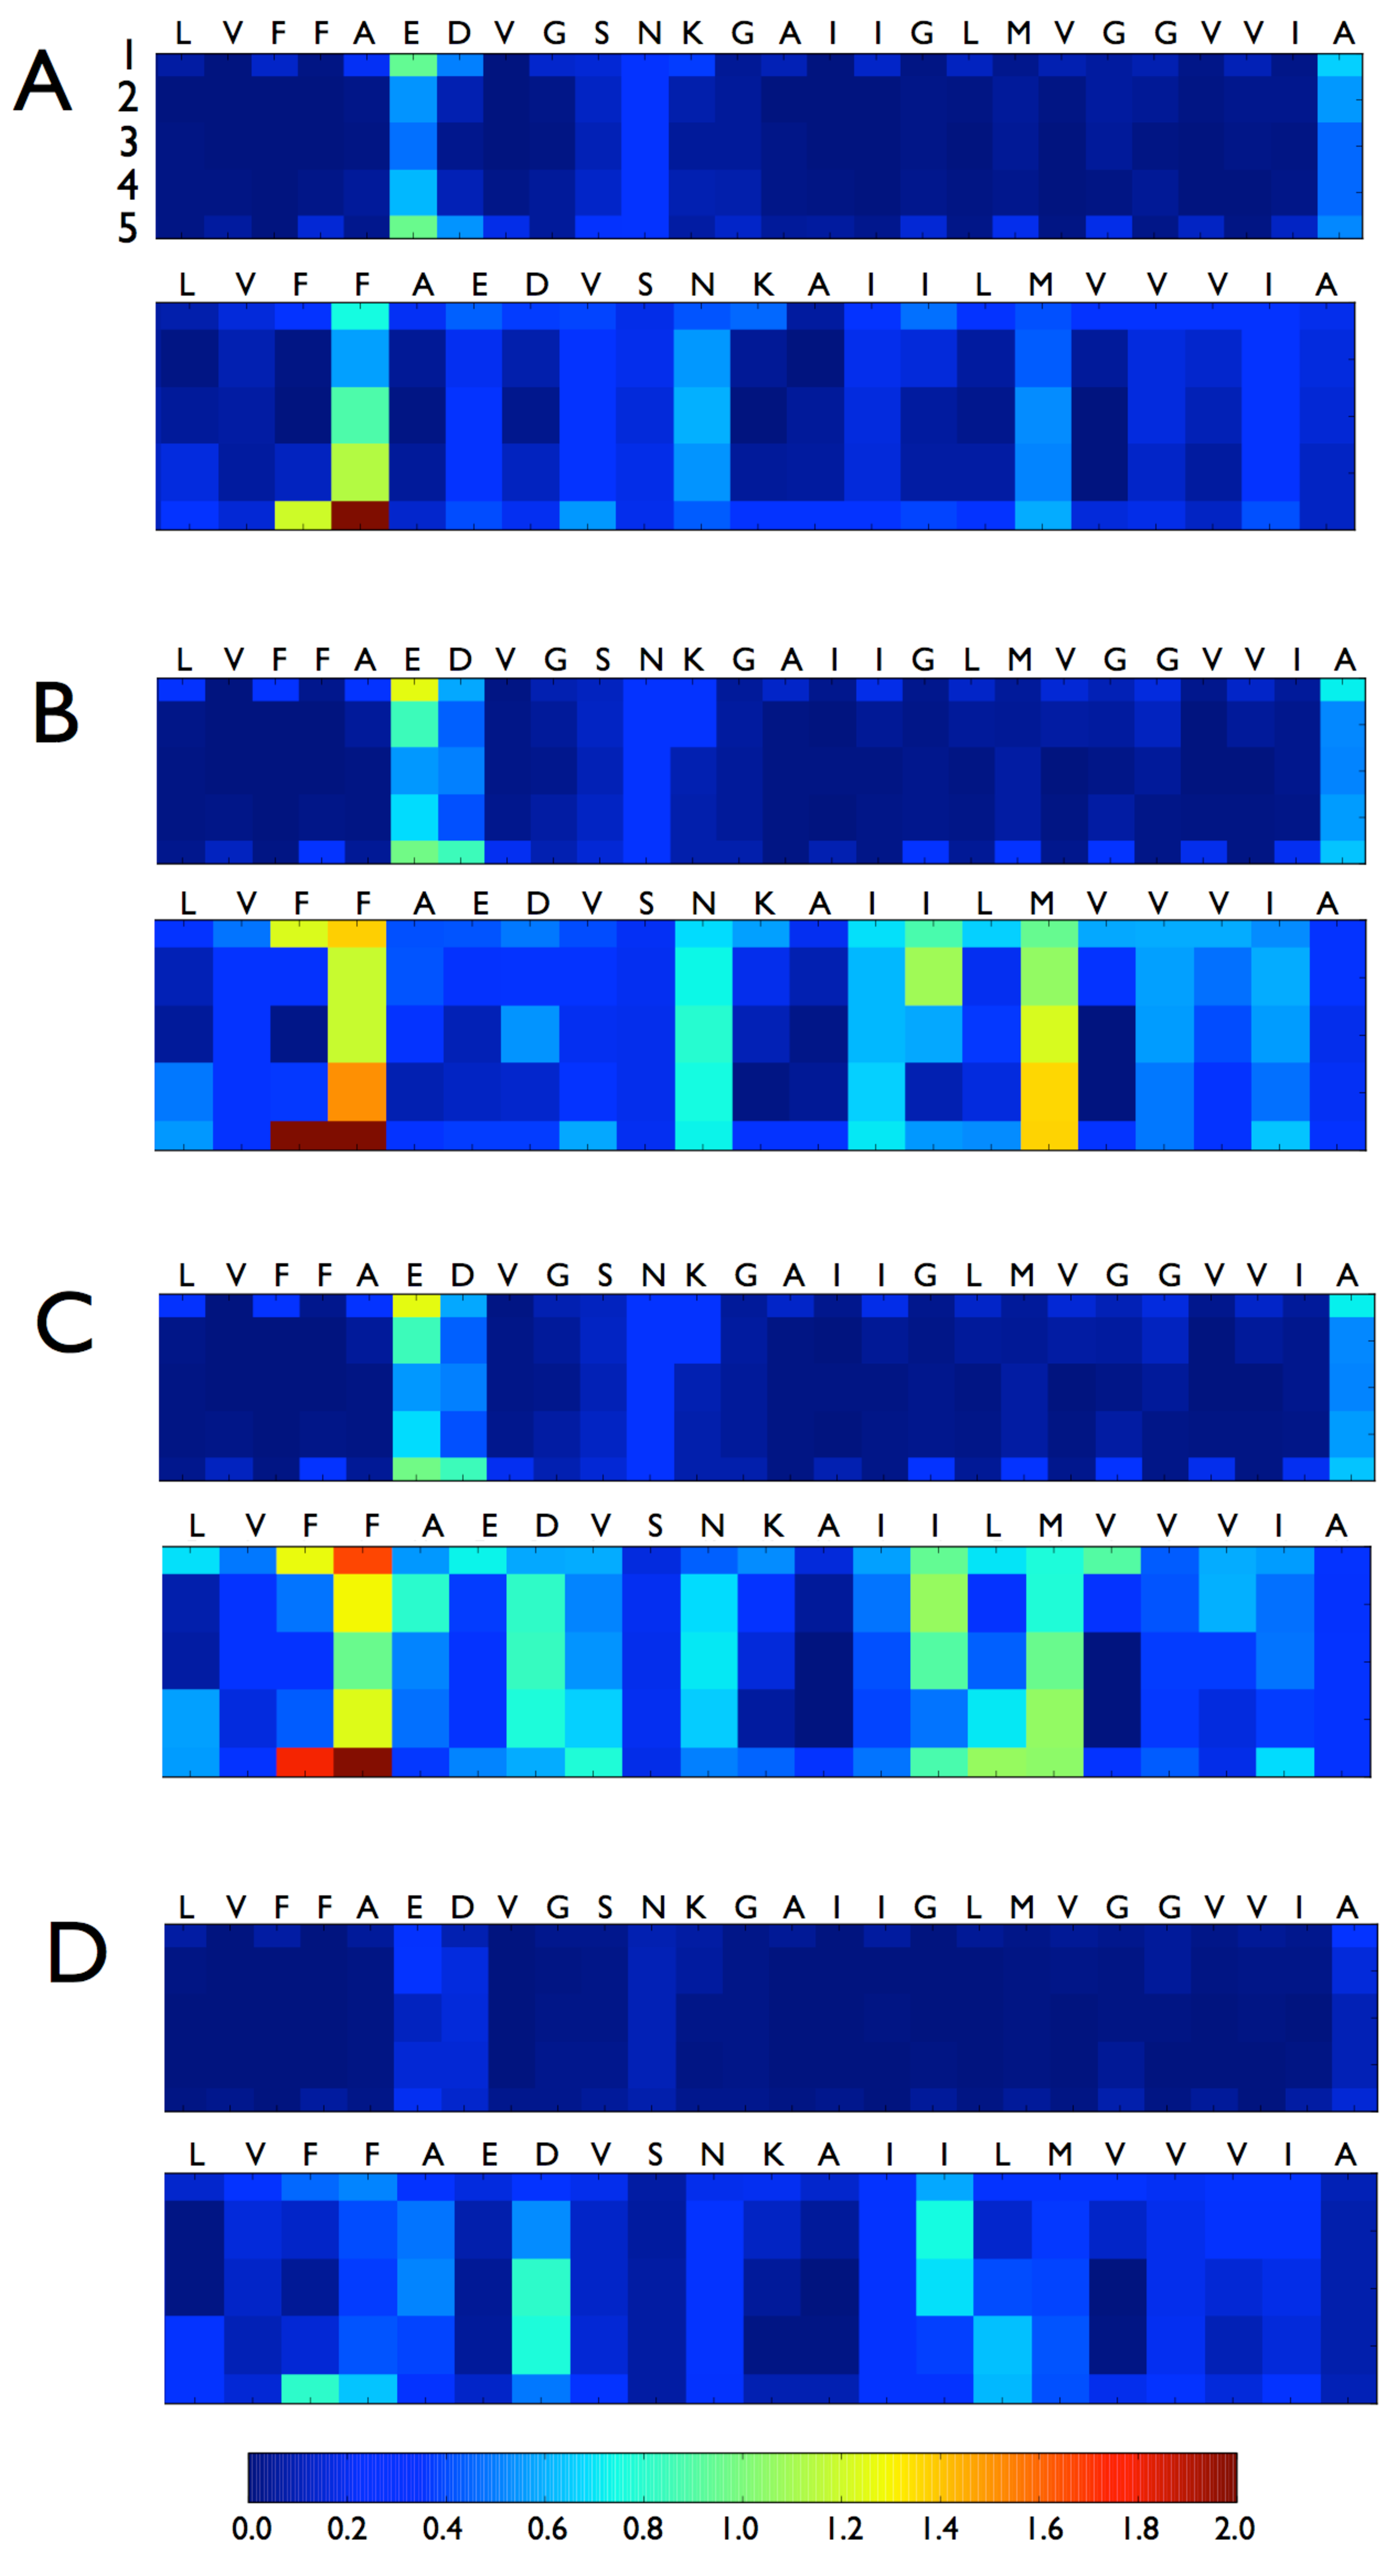
\includegraphics[width=4in]{figures/results3/binding_maps_horizontal.pdf}
  \caption[Binding contact map]{Contact maps for ligand-protofibril binding involving hydrogen bonding (top) and nonpolar contact maps (bottom) for (A) scyllo-inositol, (B) glucose, (C) chiro-inositol, and (D) glycerol. Each row and column of the matrix represents the average number of contacts for a peptide and a residue in the protofibril, respectively.}
  \label{fig:binding_map}
\end{figure}

% Binding in the channel
The protofibril exhibits a intersheet cavity surrounded by residues Asp, Lsy, Ile and Leu in the vicinity. \textbf{The cavity is formed by the stretch of residues X ...Y.  However, only the residues W Z have side chains that are exposed inside this cavity.}  A significant binding density was found for chiro-inositol, glucose, and glycerol, but not for scyllo-inositol (Figure~\ref{fig:spatial_binding}).   
% Does not happen with glycerol - completely nonspecific. Scyllo only specific to FAE region.
Both chiro-inositol and glucose molecules were found to bind to the inside of the channel by forming linearly-hydrogen-bonded chains (Figure~\ref{fig:detailed_binding_modes}), while simultaneously forming hydrogen bonds and nonpolar contacts with residues Asp, Lys, Ile, and Leu.

Although chiro-inositol and glucose were able to penetrate into the intersheet channel, scyllo-inositol was found to be mostly trapped near the channel entrance (Figure~\ref{fig:spatial_binding},\ref{fig:detailed_binding_modes}).
% Although scyllo-inositol can intercalate between the sheets near the opening of this tunnel, a significant binding density for scyllo-inositol was not found on the inside (Figure~\ref{snapshot of scyllo binding at this region}). 
In support of our results, several previous simulation studies utilizing the same model of the A$\beta$42 protofibril 
have observed similar binding modes for amyloid dye molecules (ThT and PiB),\cite{Shea} and a polyphenol morin.\cite{Lemkul et al.}
% TODO AND what???
%In corroboration with our results, a MD study by Shea et al. indicated that dye molecules, PiB and ThT,  can penetrate into the same channel for the same protofibrillar model.\cite{Wu:2011fd} (This sentence is better for discussion). -- SO WHAT?

We speculate that these binding modes are unlikely to lead to amyloid inhibition as these binding sites are not located at area where fibril growth may occur.  \textbf{These binding modes further suggest that stereochemistry }

\begin{figure}[htbp]
 \centering
 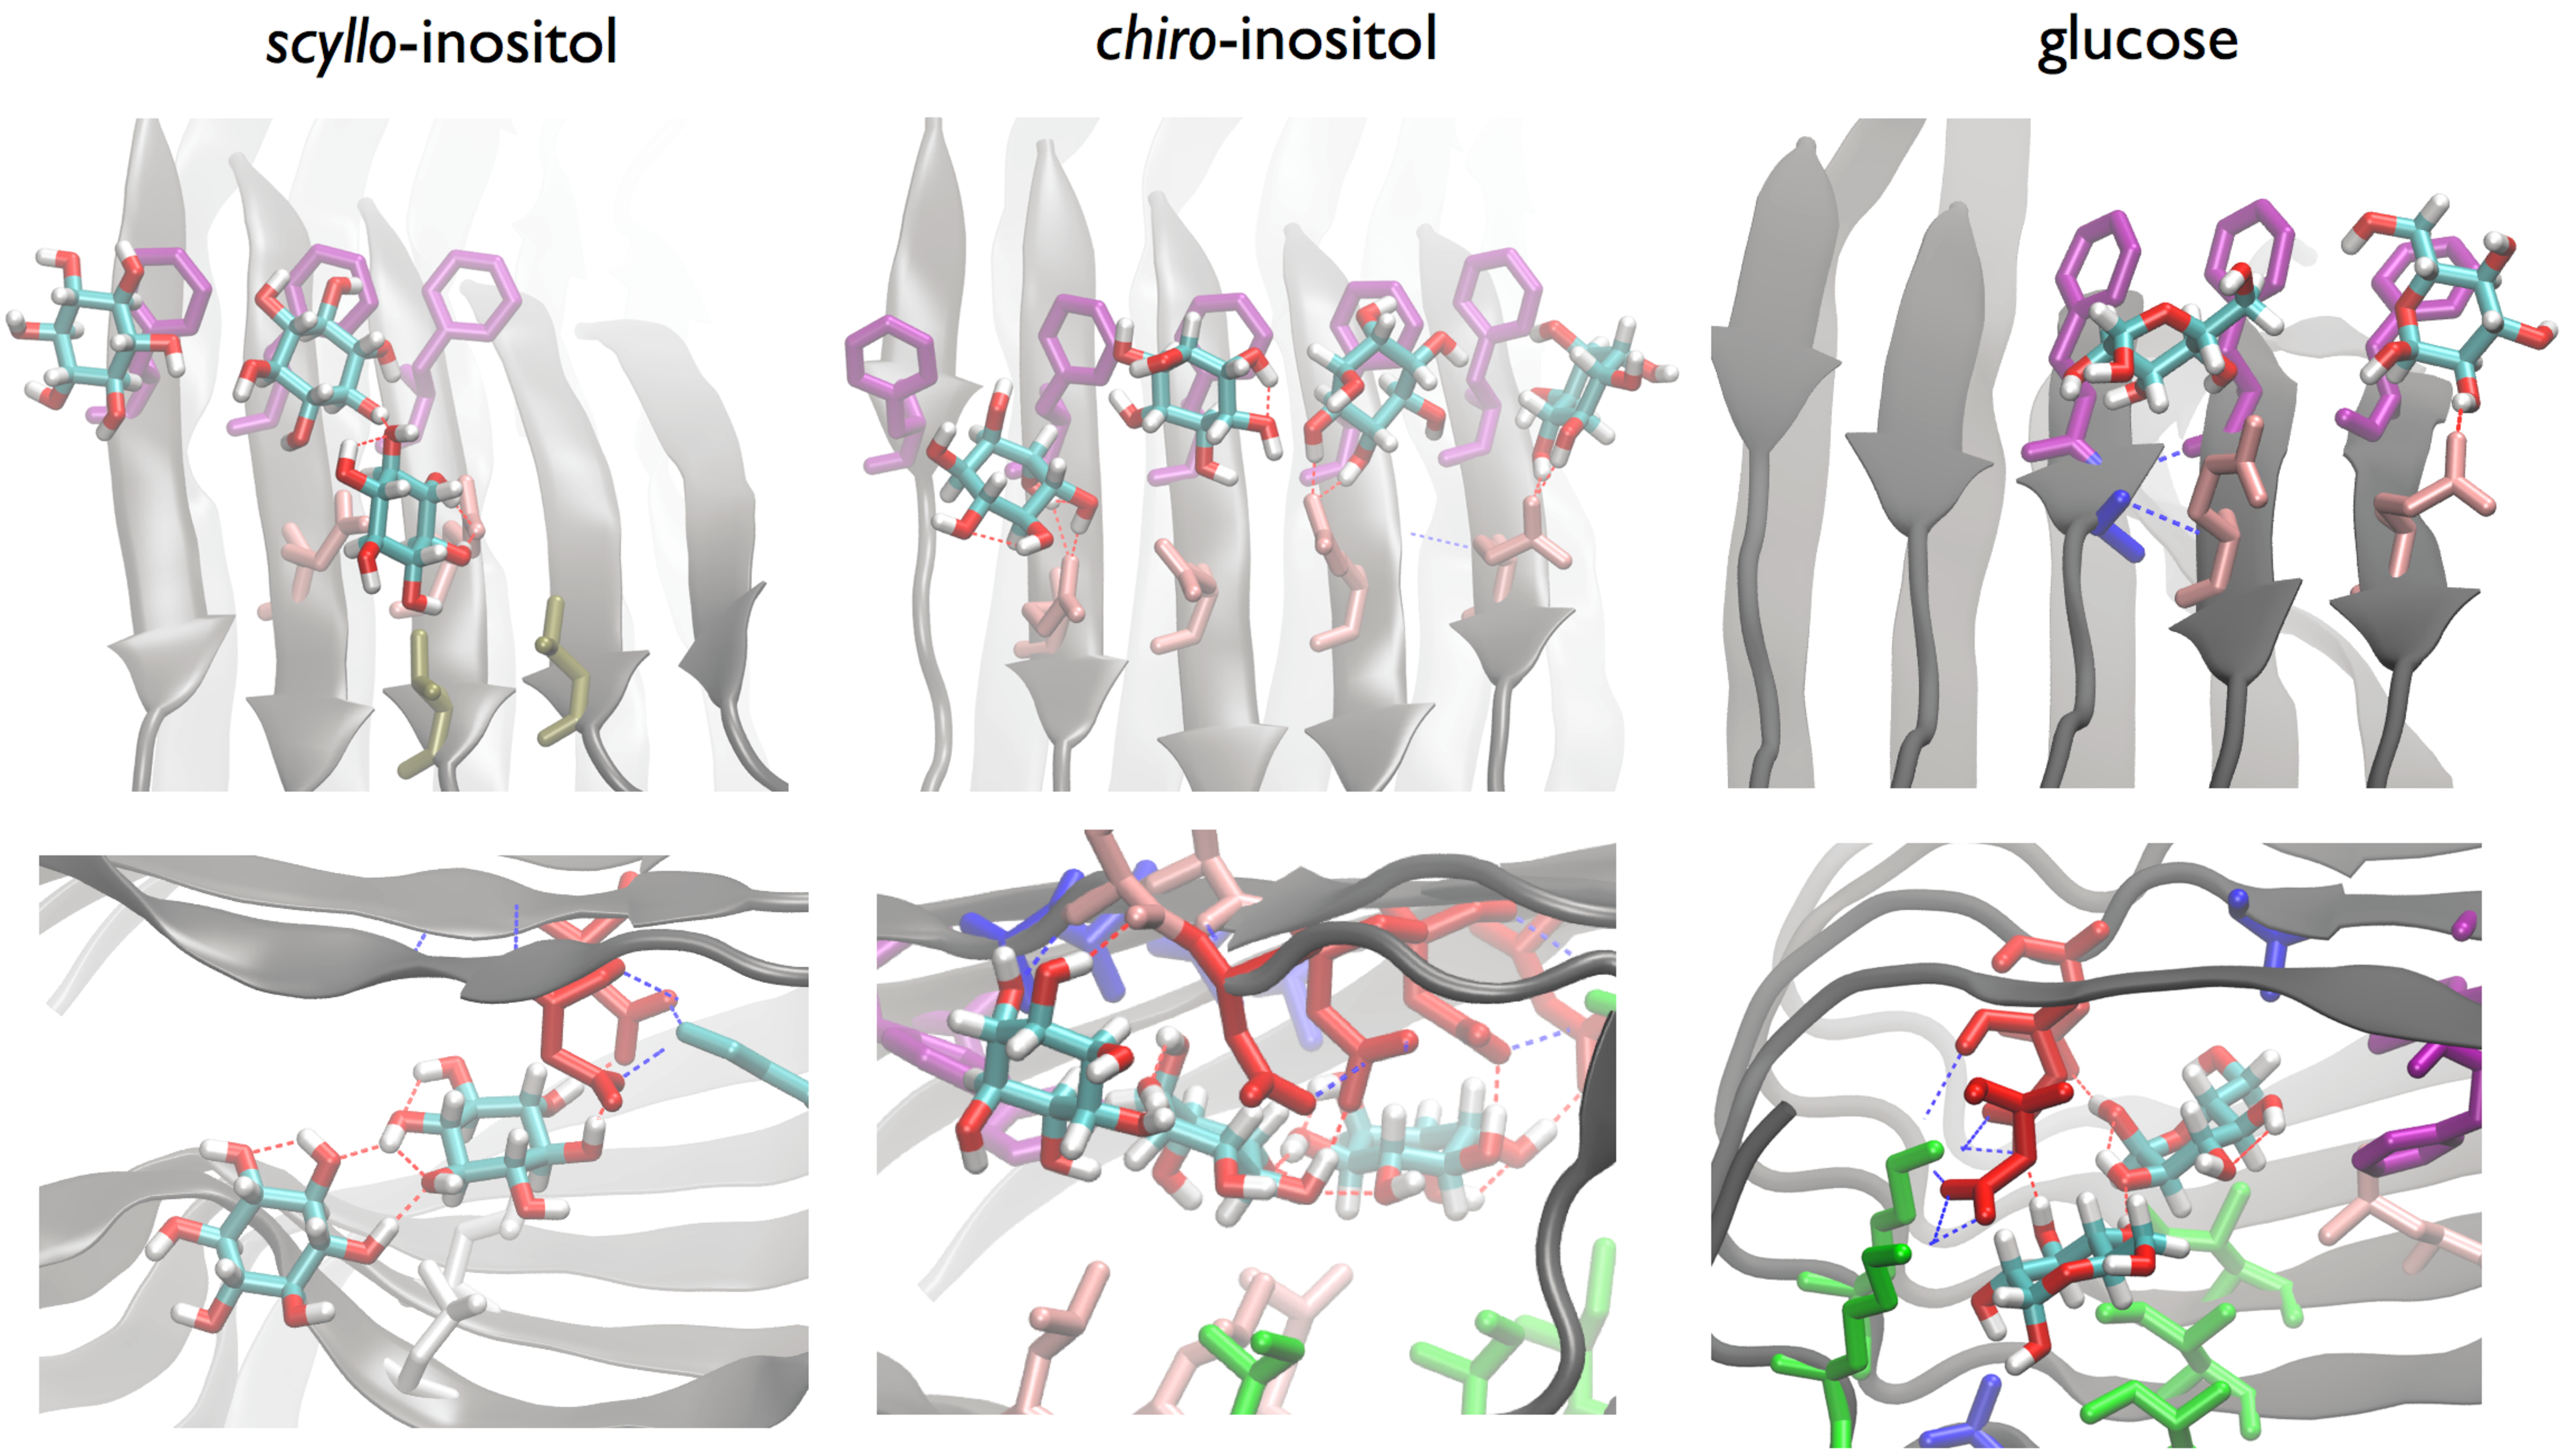
\includegraphics[width=6.5in]{figures/results3/detailed_binding_modes.pdf}
 \caption[Example binding modes of scyllo-inositol, chiro-inositol, and glucose to the protofibril]{Binding modes of scyllo-inositol, chiro-inositol and glucose to the $\beta$1 face (top row) and channel-like groove (bottom row). Residues that are within 4 \angstrom\ of a bound solute are represented in stick form. Protein is represented as a cartoon in gray.  Residues Phe, Glu, Asp, Lys and Ile are shown in colors purple, pink, red, green, and light green, respectively.}
 \label{fig:detailed_binding_modes}
\end{figure}

Ligand binding modes and binding propensity was modulated by their stereochemistry. In particular, scyllo-inositol has the highest percentage of molecules bound exclusively via hydrogen bonding.  Furthermore, bound scyllo-inositol molecules form nonpolar and hydrogen bonds in equal fractions (Figure~\ref{fig:binding_sdf_pie_chart}). By contrast, a higher fraction of chiro-inositol, glucose and glycerol molecules was found to bind by forming nonpolar contacts instead of hydrogen bonds. Furthermore, the fraction of molecules bound by nonpolar contacts increased concomitantly with a decrease in the fraction bound by hydrogen bonds for the ligands according to the following order: scyllo- (lowest), chiro-inositol, glucose and glycerol (highest) (Figure~\ref{fig:spatial_binding}). 

Consistent with the results of our previous study on KLVFFAE, our results here suggest that possessing the ability to form both hydrogen bonds and nonpolar contacts equally favorably may be an important property of small molecules (to target the CHC) and therefore, ultimately, for the inhibition of amyloid formation.
% Elaborate -- what are the implications of this finding?  Are there current papers which suggests this?  In my inos2 paper, I mentioned this and RP mentioned that this is really what is coming out of this study. Maybe discuss this in more detail than what was covered in inos2 ...
% Discuss the trend where scyllo, chiro, glucose, and glycerol have increasing nonpolar-only contacts and decreasing polar only contacts, but nonpolar and polar remained relatively stable.

% Our previous study indicated that the balance of nonpolar and hydrogen bonding interactions is important (and dictates the binding specificity!!!) in inositol binding to monomer and aggregates of the peptide KLVFFAE because that is where scyllo and chiro differed in their binding modes.
% Solutes were also found to bind to the residues located in the turn region (on the surface). This and binding inside the tunnel are binding modes that are unlikely to be involved in amyloid inhibition.

\begin{figure}[htbp]
  \centering
  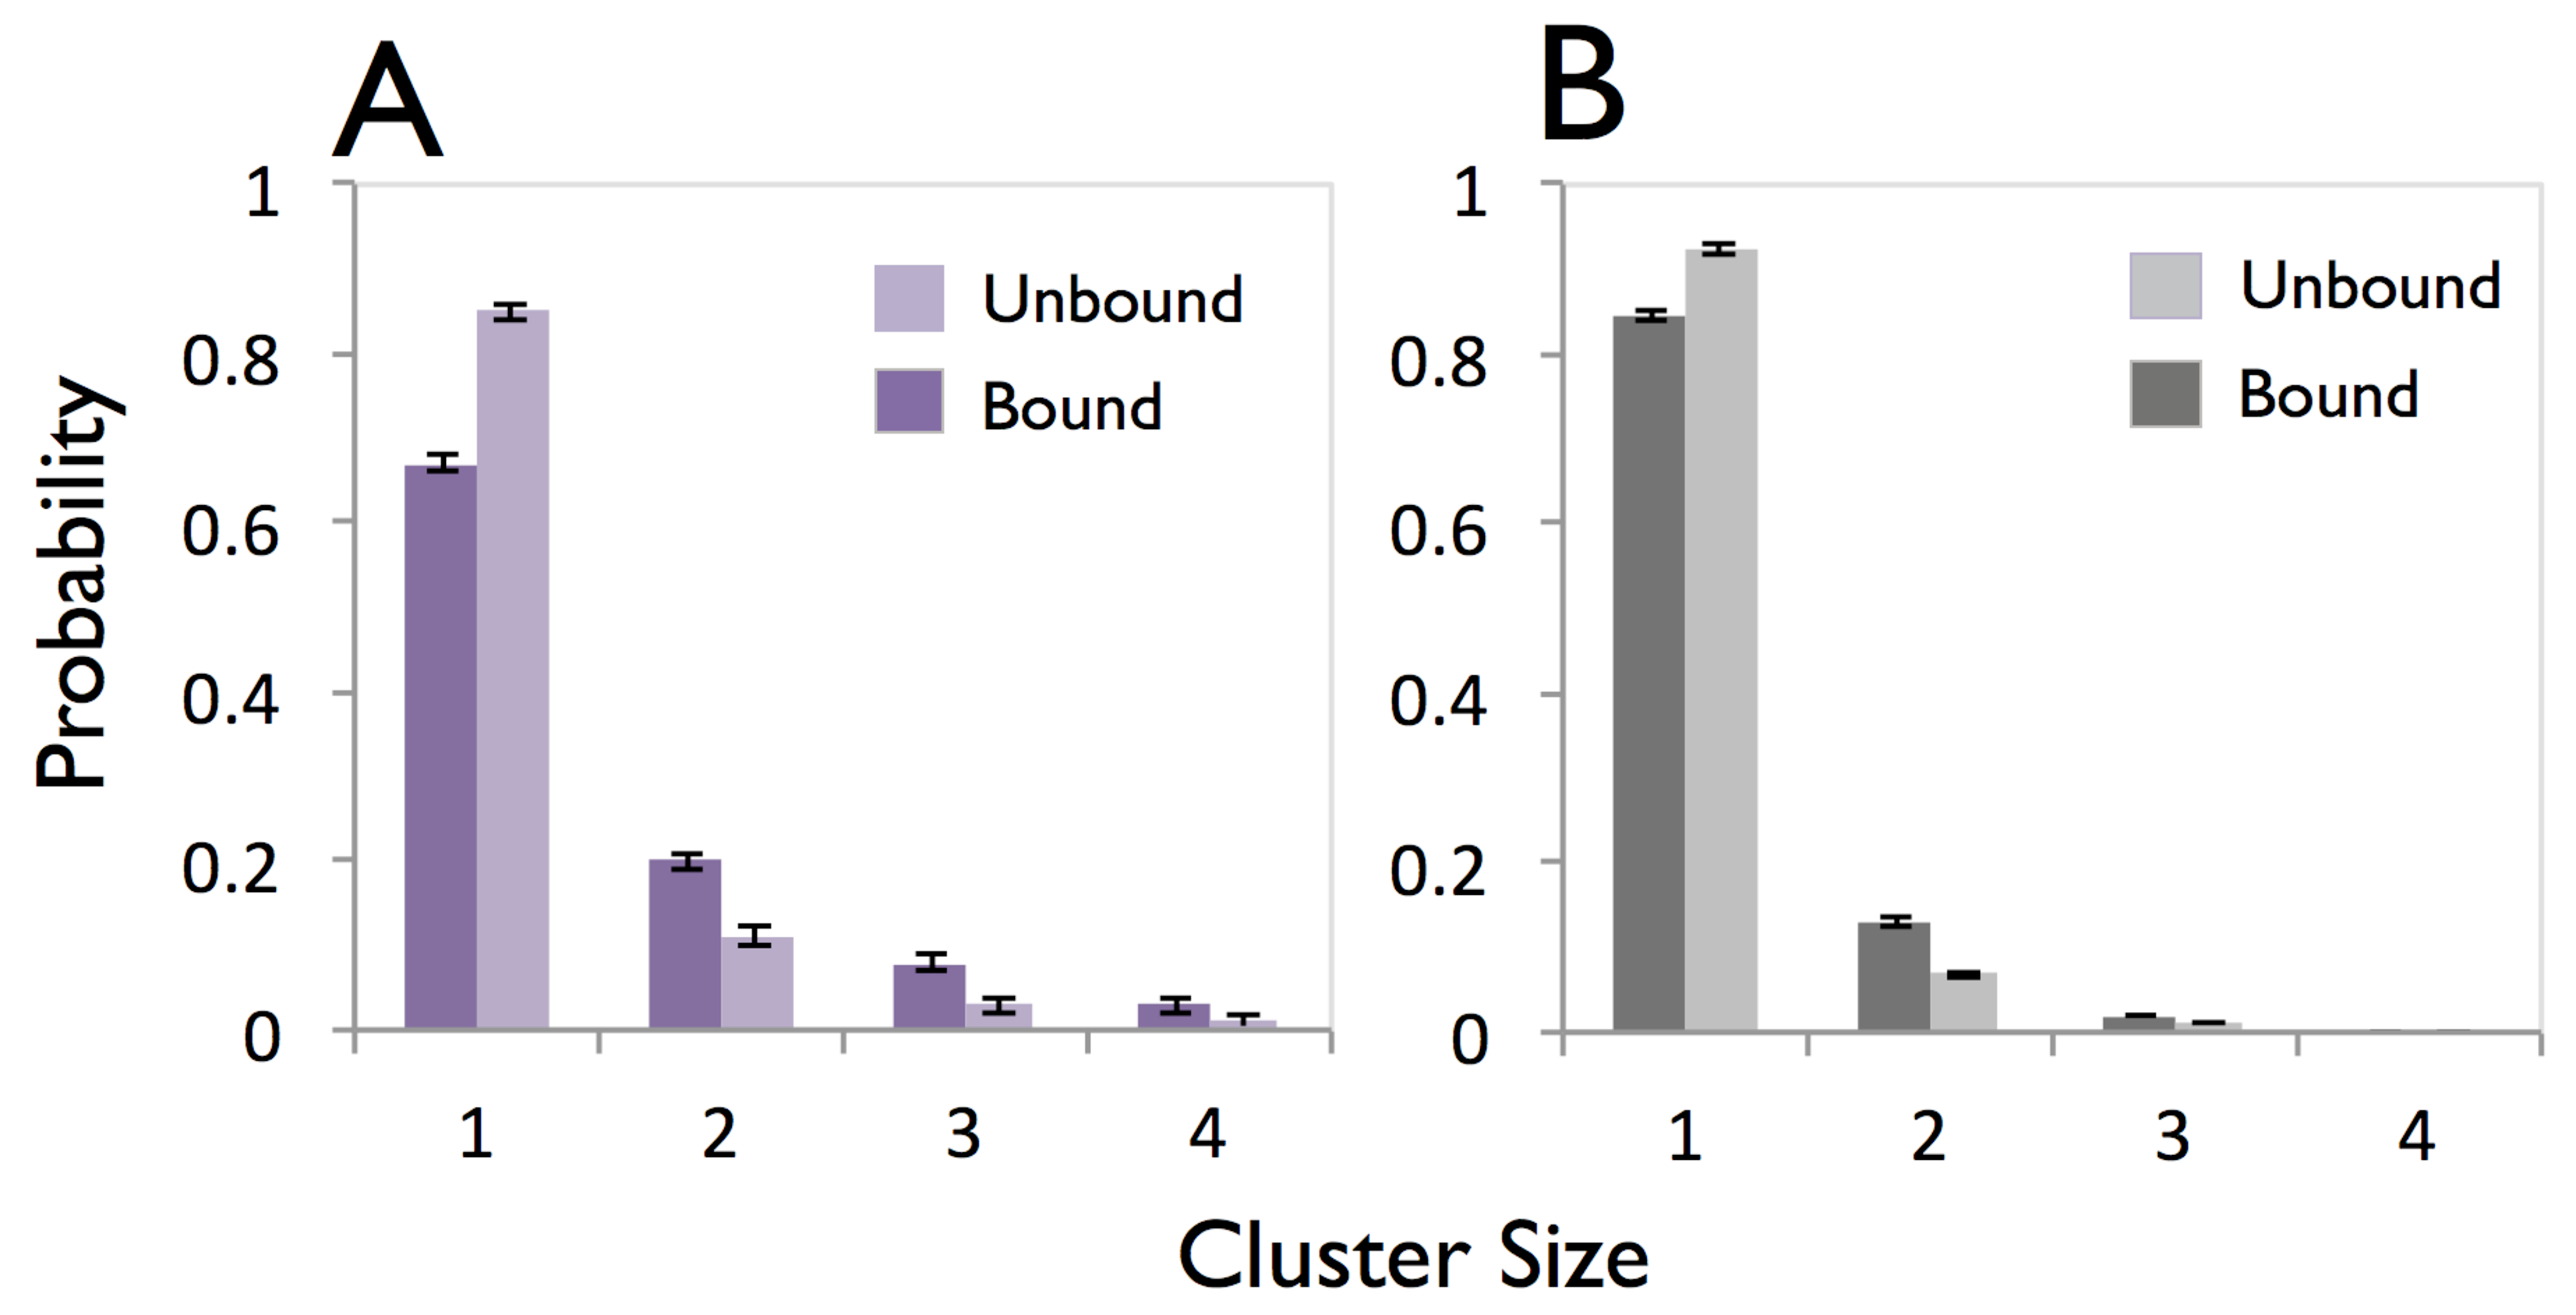
\includegraphics[width=6in]{figures/results3/clustered_binding.pdf}
  \caption[Clustered binding of solutes at the surface of the protofibril]{Bound versus unbound cluster histograms for each solute.}
  \label{fig:cluster_binding}
\end{figure}

Consistent with our previous study,\cite{Li:2013}, inositol bound to the surface of the Abeta protofibril in clusters (Figure~\ref{fig:cluster_binding}. Within a cluster, ligand molecules form self-interactions via intermolecular hydrogen bonds and nonpolar contacts. Examples of such binding modes are show in Figure~\ref{fig:XXX}. Our results here are consistent with our previous study with A$\beta$(16-22)\cite{Li:2013}.  In that study, inositol was found to bind to amyloid fibrils in a supramolecular form, which suggested this binding mode may play a role in amyloid inhibition by small molecules.  In corroboration with our studies, these results  have been observed in simulation studies by Shea and co-workers, and experimentally for CR binding (37) by Kr�l and co- workers.\textbf{REF}  Although the distribution of cluster sizes for glycerol suggests that it is less likely than the other ligands for forming clusters when bound, there was no difference in the distribution between chiro-, scyllo-inositol, and glucose. 

\subsection{Molecular basis of amyloid inhibition by \textit{scyllo}-inositol}
% or \subsection{Implications for amyloid inhibition of A$\beta$42 by inositol}

\subsection{Comparison with binding to the protofibril of A$\beta$(16-22)}
\textbf{Have a paragraph discussing the consistency of results here and the results in my previous studies.  I'm being too repetitive if I mention that it's consistent with KLVFFAE after every results and discussion paragraph}

\section{Discussion}
% - Binding specificity of inositol
%  - mention binding to FAE - but why?; should have a discussion of amyloid inhibition based on the observed binding modes;
% -  discussion of how the full length binding compares with KLVFFAE binding - impt mention that the binding modes are consistent in all models - comforting result

% Comment on MD simulations as a technique as a whole for understanding these types of interactions -- should this be a discussion point? -- maybe move this to conclusions  

The spatial binding probability distribution, depicted in Figure~\ref{fig:spatial_binding}, suggests that scyllo-inositol has the highest preference for the face of the protofibril containing the residues found in the central hydrophobic core (CHC) of A$\beta$, LVFFAE, particularly to the residues F-A-E. By contrast, inactive molecules, chiro-inositol and glucose were both found to predominantly partition to the $\beta$2 face.  \textbf{What is the reason for this?} 
There are a few reasons. In our previous study, we demonstrated that scyllo-inositol displays higher binding specificity to phenylalanine: scyllo-, but not chiro-inositol, adopts a face-to-face binding mode with phenylalanine. By contrast, due to stereochemistry differences, chiro-inositol and glucose molecules do not possess such a binding mode. Consistent with this result, both chiro-inositol and glucose possessed spatial distributions that were more wider spread than that of scyllo-inositol, indicating that they display less binding specificity. 
% Their binding is less specific to the same region than that of scyllo-inositol.  
Taken together, our results indicate that the binding specificity of scyllo-inositol is to the amyloidogenic core of A$\beta$ amyloid. This is consistent with what we found in our KLVFFAE study.

On the basis of our results, we hypothesize that binding to the face of protofibrils containing the residues LVFFAE may be a productive small-molecule binding mode for the inhibition of lateral stacking of fibrils.  The difference in the binding specificity of scyllo- and chiro-inositol towards the $\beta$1 face may explain the differences between the activity of scyllo- and chiro-inositol in the inhibition of A$\beta$ amyloid fibrillation.  Because of it's binding specificity, scyllo- may prevent the lateral association of fibrillar aggregates by binding to the $\beta$1 face. Without the ability to stabilize the cross-$\beta$ structure by stacking laterally, single-layered protofibrillar structures are unlikely to propagate into mature fibrils. 
%which ultimately lead to inhibition of amyloid formation.. % ie. require stacking to grow into the long unbranched morphology seen in EM.

Many lines of evidence suggests that KLVFFAE is responsible for fibril formation (REF: de groot) (experimental studies?). The CHC is thought to be responsible for the initiation of A$\beta$42 aggregation and $\beta$-sheet formation. Furthermore, our previous studies indicated that the likely mode of action of inositol is to binding to surfaces of $\beta$-sheets, specifically those involving the KLVFFAE segment.\cite{inos1, inos2}
On the basis of our results above, we hypothesize that the CHC, particularly the region spanned by the residues Phe20 and Glu21, is a critical target for destabilizing A$\beta$42 fibrils. This is supported by the results of other simulation studies. Convertino et al.\cite{convertino} where anthraquinone was observed to bind to the peptide QLVFFA region. This binding mode is likely modulated by the stereochemistry and physicochemical properties of the small molecule. For example, in a simulation study of morin binding to A$\beta$42 by Lemkul et al., morin which is a polyphenol molecule with multiple phenol rings forming a planar geometry, was not found to bind to this region of the protofibril.

% Both Joanne and Mark said tonnes of literature supporting this face is relevant for inhibition!!!  --- where is this literature?
% Thus far, our results suggest that  scyllo best (or rather more specifically) to this face. This is an interesting conclusion / difference that thus only could tell from from the abeta42 model because it has two different faces which brought out the preferential binding of scyllo to the KLVFFAE face.
Our results are consistent with these studies and supports the hypothesis that selectively targeting the CHC segment of the A$\beta$ may be a viable approach for the inhibition of A$\beta$ fibrillation.
% Taken together, our results suggest that selectively targeting the CHC \textbf{is a good approach for developing potential amyloid inhibitors}.

% Scyllo- binds this face better than chiro-, glucose, and glycerol inactive solutes in fibril inhibition.  
% We speculate (is it speculation?) that the activity of scyllo-inositol in the inhibition of fibril formation is due to its preference for binding to the $\beta$-sheet face of the protofibril involving the residues in the CHC of \ab42. 
% Furthermore, we speculate that scyllo-inositol is active because it adopts more inhibition-productive binding modes than both chiro-inositol and glucose. Consistent with these results, our previous studies have indicated that scyllo-inositol binds with higher specificity with nonpolar groups of A$\beta$(16-22) than chiro-inositol. \textbf{For example, when chiro-inositol binds inside of the channel is a ``non-productive'' binding modes.} - Not sure if any of these are based on any results.


% Comment on how good are these model peptides for understanding inhibitor binding interactions. Do I really want to discuss this? I think this is better to discuss in my thesis conclusions?
Comparisons to binding to the beta-oligomer of KLVFFAE - Depending on the morphology of the amyloidogenic aggregate, the binding modes can be different. In our previous study, we examined binding with KLVFFAE. Because KLVFFAE has identical faces, the preferential binding to KLVFFAE was not revealed.  The surface of KLVFFAE consists of both polar, charged and hydrophobic pockets, whereas the grooves on the surface of the oligomer are largely hydrophobic. 
% The core of the abeta42 fibril solved by Luhrs et al. protofibril of the Abeta42 can be thought of as an early beta-sheet oligomer of Abeta42. 
% Binding modes with aggregates of model abeta peptides may have modes that differ from the full length amyloid. 
%It may have been that for this reason, we observed that both scyllo and chiro were bound with similar Keq to the protofibril of KLVFFAE.  
% However, with differing faces on the Abeta protofibril, we were  able to identify preferential binding of scyllo- to the KLVFFAE face.
Moreover, another difference between the protofibrils of KLVFFAE and full-length Abeta is the appearance of new binding modes which were observed with the Abeta, but not the KLVFFAE protofibril. \textbf{There are other binding modes .. some does not seem productive. It seems like non-inhibitors like glucose and chiro- are more prone to participating in these binding modes} Although small molecules can bind inside the protofibril, these binding modes do not disrupt the integrity of the protofibril. We hypothesize that binding in this region may be an unproductive binding mode, which may decrease the activity of small molecules. 
% We speculate that because scyllo-inositol is not trapped by unproductive binding modes, this may explain why scyllo-, but not chiro-inositol, is active in the inhibition of \ab42. - Not so sure about this idea.
Based on our results, it shows that it is useful to comparatively examine protofibrils to determine true binding modes of a drug. And that drugs may have differential effects for different peptide sequences.

\textbf{The discussion of why not Abeta40 but Abeta42 should be included at the end of the discussion section as this is going to be quite speculative - it may be because of differing binding modes due to differences in fibril structure}. However, further studies that are similar to the current study will be needed to elucidate differences in their binding. 
% In addition to stereochemistry-dependent activity, inositol was found to be inactive for inhibiting the amyloid formation of Abeta40 - put forth a few speculations based on the data of my current study to explain.  

% \textbf{More speculative - Relevance of the NMR models.} I can say something about the suggested accuracy of the NMR models based on my sim. results?  Radius of gyration? The model falls apart? Does this mean that the NMR model is not ``right'' ? Is the pentamer a stable unit of the fibril ? ``accuracy'' of the NMR models -- how good are these models?  It is unlikely I'm going to be able to say much here, we have no idea what the actual experimental stability of this species is.  This pentamer fragment may not be stable on its own, but could be just a building block in a stable extended fibrillar structure of A$\beta$42. -- But based on my recollection a study by Masman sugggests that this is the stable core. - I'm not sure if this is a useful thing to have in my discussion


% Whole idea:  binding at the surface and preventing stacking, rather than insertion.  Insertion is not likely to be a productive binding mode for inhibition. Why? because I don't observe disruptive insertion (I need to define this) - scyllo doesn't really insert, chiro- does, but no disruption to the aggregate ...
% More quantitatively I probably _need_ to quantify affinity to the KLVFFAE face of the Abeta fibril for scyllo chiro, glucose
% Also should do epi.  But what if epi does not bind to KLVFFAE face? How would I then explain that epi is also active but does not go to KLVFFAE? This could disprove my entire hypothesis ... though its not likely because chiro goes to the KLVFFAE face.
% I think a Shea paper talks about the importance of preventing stacking


\section{Conclusions}
No difference in the fibril conformations with and without inositol in either the low or high molar ratio simulations. Does glucose bind more or less? If it does bind less, then it tells us that we might be onto something with scyllo-inositol even though the structure is subtly different.  Glucose does not necessarily bind ``less", but it does not bind on the right face ie. the KLVFFAE face Scyllo-inositol appears to preferentially bind the KLVFFAE face, more than glucose and chiro-inositol.  Furthermore scyllo does not bind in a hydrated tunnel formed in the protofibrillar aggregate.  Binding mode differences between active and inactive inhibitors of  Abeta suggest a mechanism of inhibition.

\section{Acknowledgements}
% We thank Drs. JoAnne McLaurin, Mark Nitz and Chris Neale for reading the manuscript and for providing insightful comments. 
This work was made possible by the GPC supercomputer at the SciNet HPC Consortium and Compute/Calcul Canada (Colosse CLUMEQ). This work was supported in parts by the Canadian Institutes of Health Research (Grant No. MOP84496). R.P. is a CRCP chairholder.

% \section*{Supporting Information Available}
% Binding mode analyses of inositol with monomeric and aggregate systems at inositol concentrations and inositol:peptide molar ratios that were not shown in the main text; Analyses of peptide self-aggregation for the formation of the disordered oligomer; Snapshots of the starting simulation structure of the $\beta$-oligomer. Supporting Information Available: Full description of the material. This material is available free of charge via the Internet at http://pubs.acs.org.

%http://www.pnas.org/content/102/2/315.full
%Support for the Significance of the LVFFA binding:
% The central hydrophobic cluster of amyloid-β (residues 17–21 LVFFA) has been particularly implicated in amyloid fibril formation (19). Tjernberg et al. (20) found that the fragment QKLVFF binds to amyloid β to prevent amyloidogenesis, whereas follow-up studies investigated the short peptides, LVFFA (21) and LPFFD (22), and showed that they are also inhibitors and that the fragment KLVFFAE forms well ordered fibrils. 
%
%KLVFFA binds to ABeta42 -- do they where they bind?
%Tjernberg, L. O., Naslund, J., Lindqvist, F., Iohansson, J., Karlstrom, A. R., Thyberg, J., Terenius, L., and Nordstedt, C. (1996) Arrest of ������-amyloid fibril formation by a pentapeptide ligand, J. Biol. Chem. 271, 8545-8548.
%
%
%Second, Aβ(16-22) peptide, which includes the central HP core, CHC (LVFFA), is recognized as being essential for Aβ fibrillation (27,28) and also forms amyloid fibrils with antiparallel β-strands in isolation (29). Third, the KLVFF motif is a primary target in the search for aggregation inhibitors for AD therapeutics (30,31).
%28. Nilsberth C., Westlind-Danielsson A., Lannfelt L. The ‘Arctic’ APP mutation (E693G) causes Alzheimer's disease by enhanced Aβ protofibril formation. Nat. Neurosci. 2001;4:887–893. [PubMed]
%29. Balbach J.J., Ishii Y., Tycko R. Amyloid fibril formation by A β 16-22, a seven-residue fragment of the Alzheimer's β-amyloid peptide, and structural characterization by solid state NMR. Biochemistry. 2000;39:13748–13759. [PubMed]
%30. Lowe T.L., Strzelec A., Murphy R.M. Structure-function relationships for inhibitors of β-amyloid toxicity containing the recognition sequence KLVFF. Biochemistry. 2001;40:7882–7889. [PubMed]
%31. Lashuel H.A., Hartley D.M., Callaway D.J. New class of inhibitors of amyloid-β fibril formation. Implications for the mechanism of pathogenesis in Alzheimer's disease. J. Biol. Chem. 2002;277:42881–42890. [PubMed]
% \section*{Figures}

%\begin{figure}[htbp]
%  \centering
%  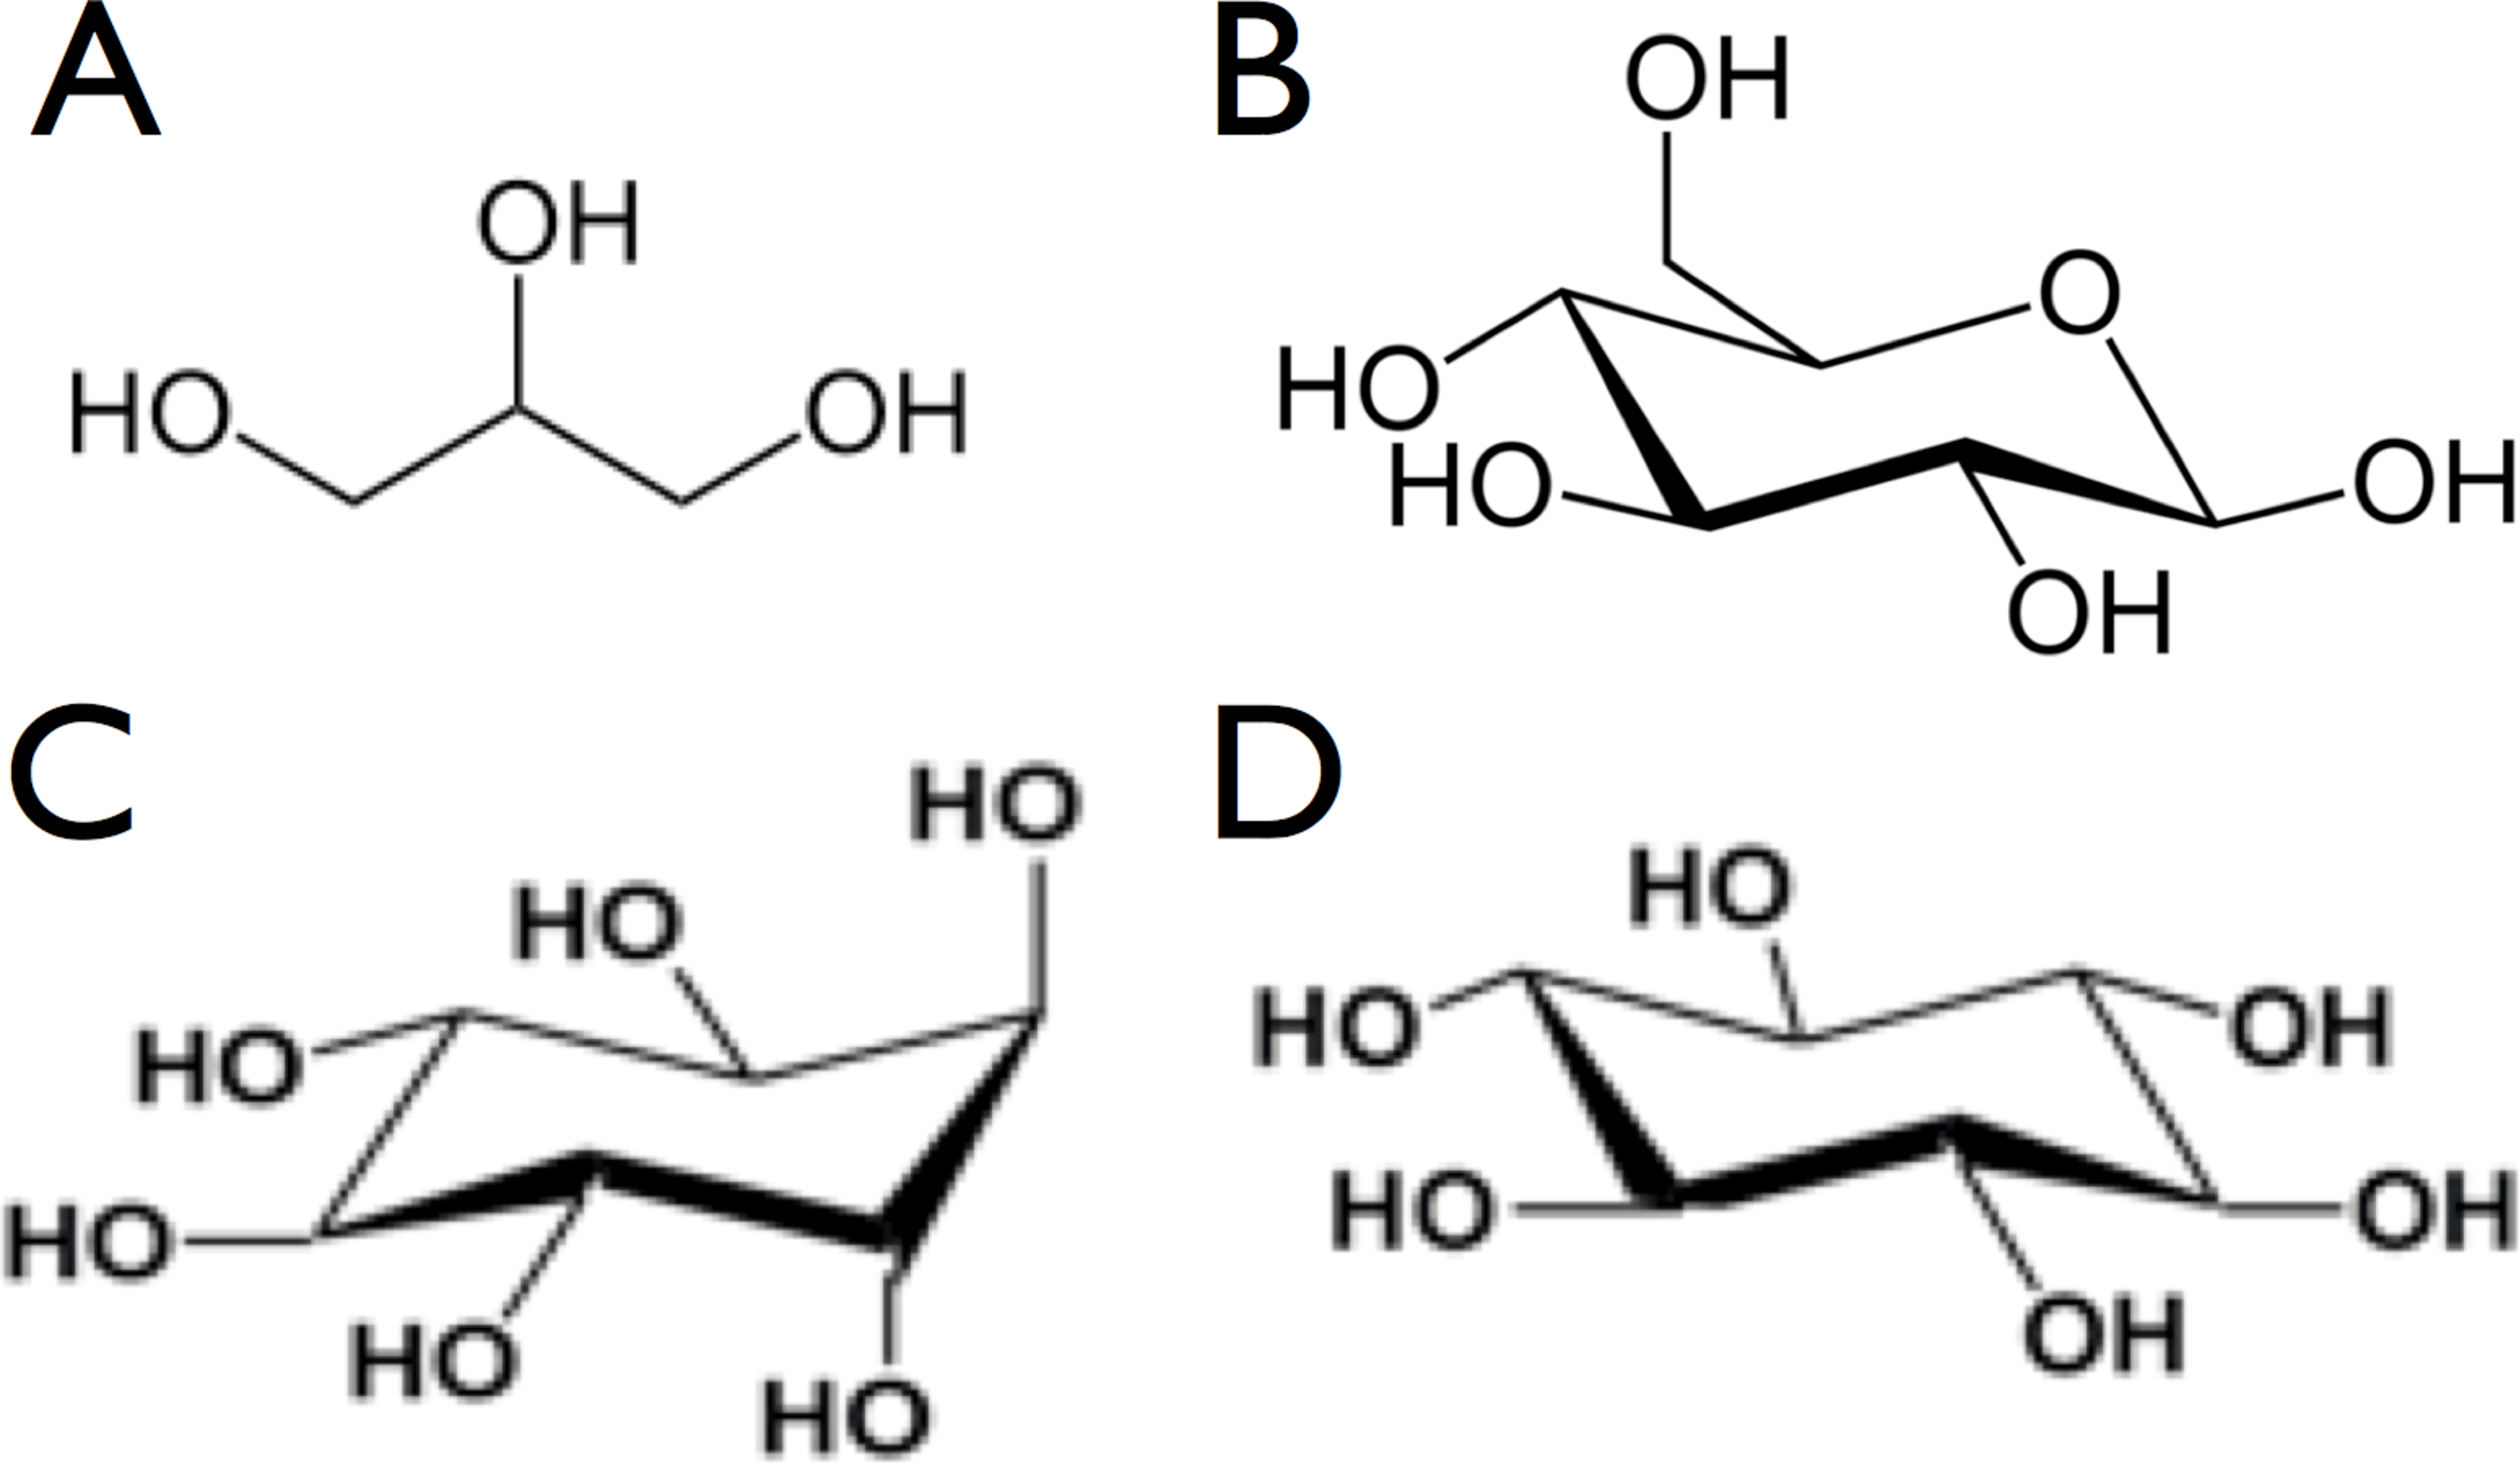
\includegraphics[width=2.5in]{figures/results3/ligands.pdf}
%  \caption[Ligands]{Molecular structures of (A) glycerol, (B) glucose, (C) chiro-inositol and (D) scyllo-inositol}
%  \label{fig:ligands}
%\end{figure}
%
%\begin{figure}[htbp]
%  \centering
%  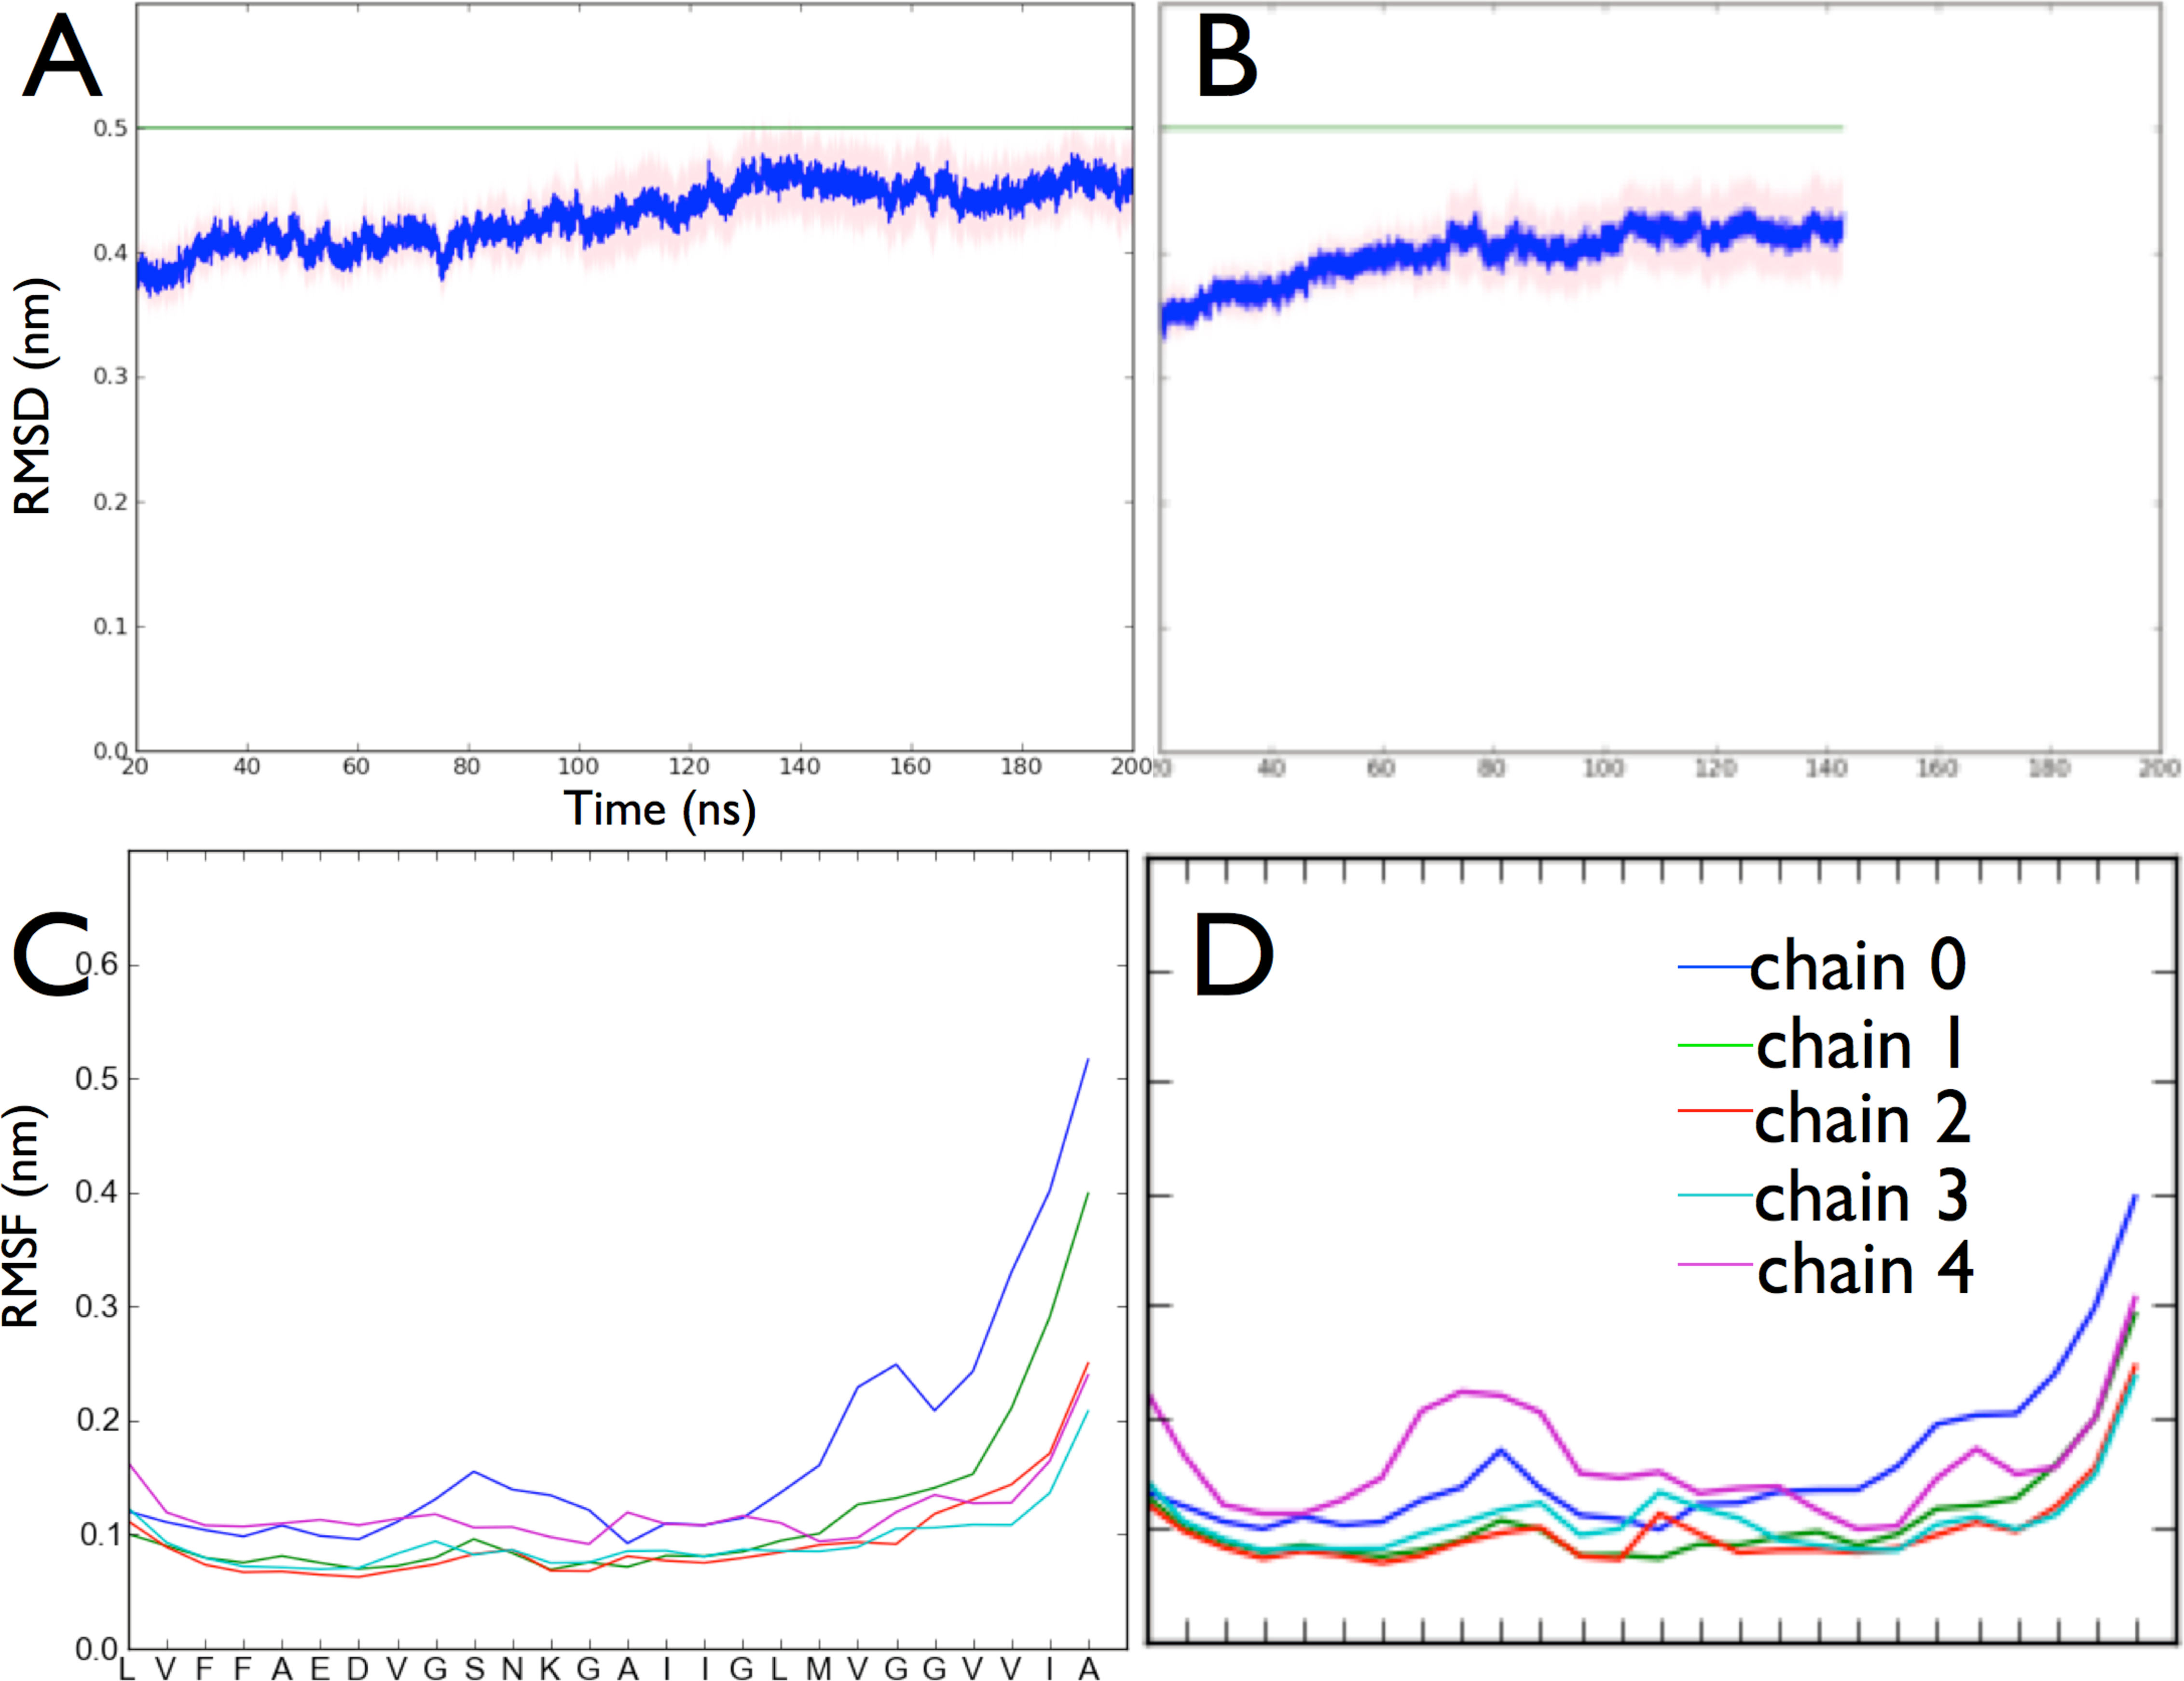
\includegraphics[width=5in]{figures/results3/protofibril_dynamics.pdf}
%  \caption[RMSD and RMSF vs. time]{Fibril structure dynamics in pure water (A) and (C), and in the presence of scyllo-inositol (B) and (D).}
%  \label{fig:protofibril_dynamics}
%\end{figure}

%\begin{figure}[htbp]
% \centering
 % 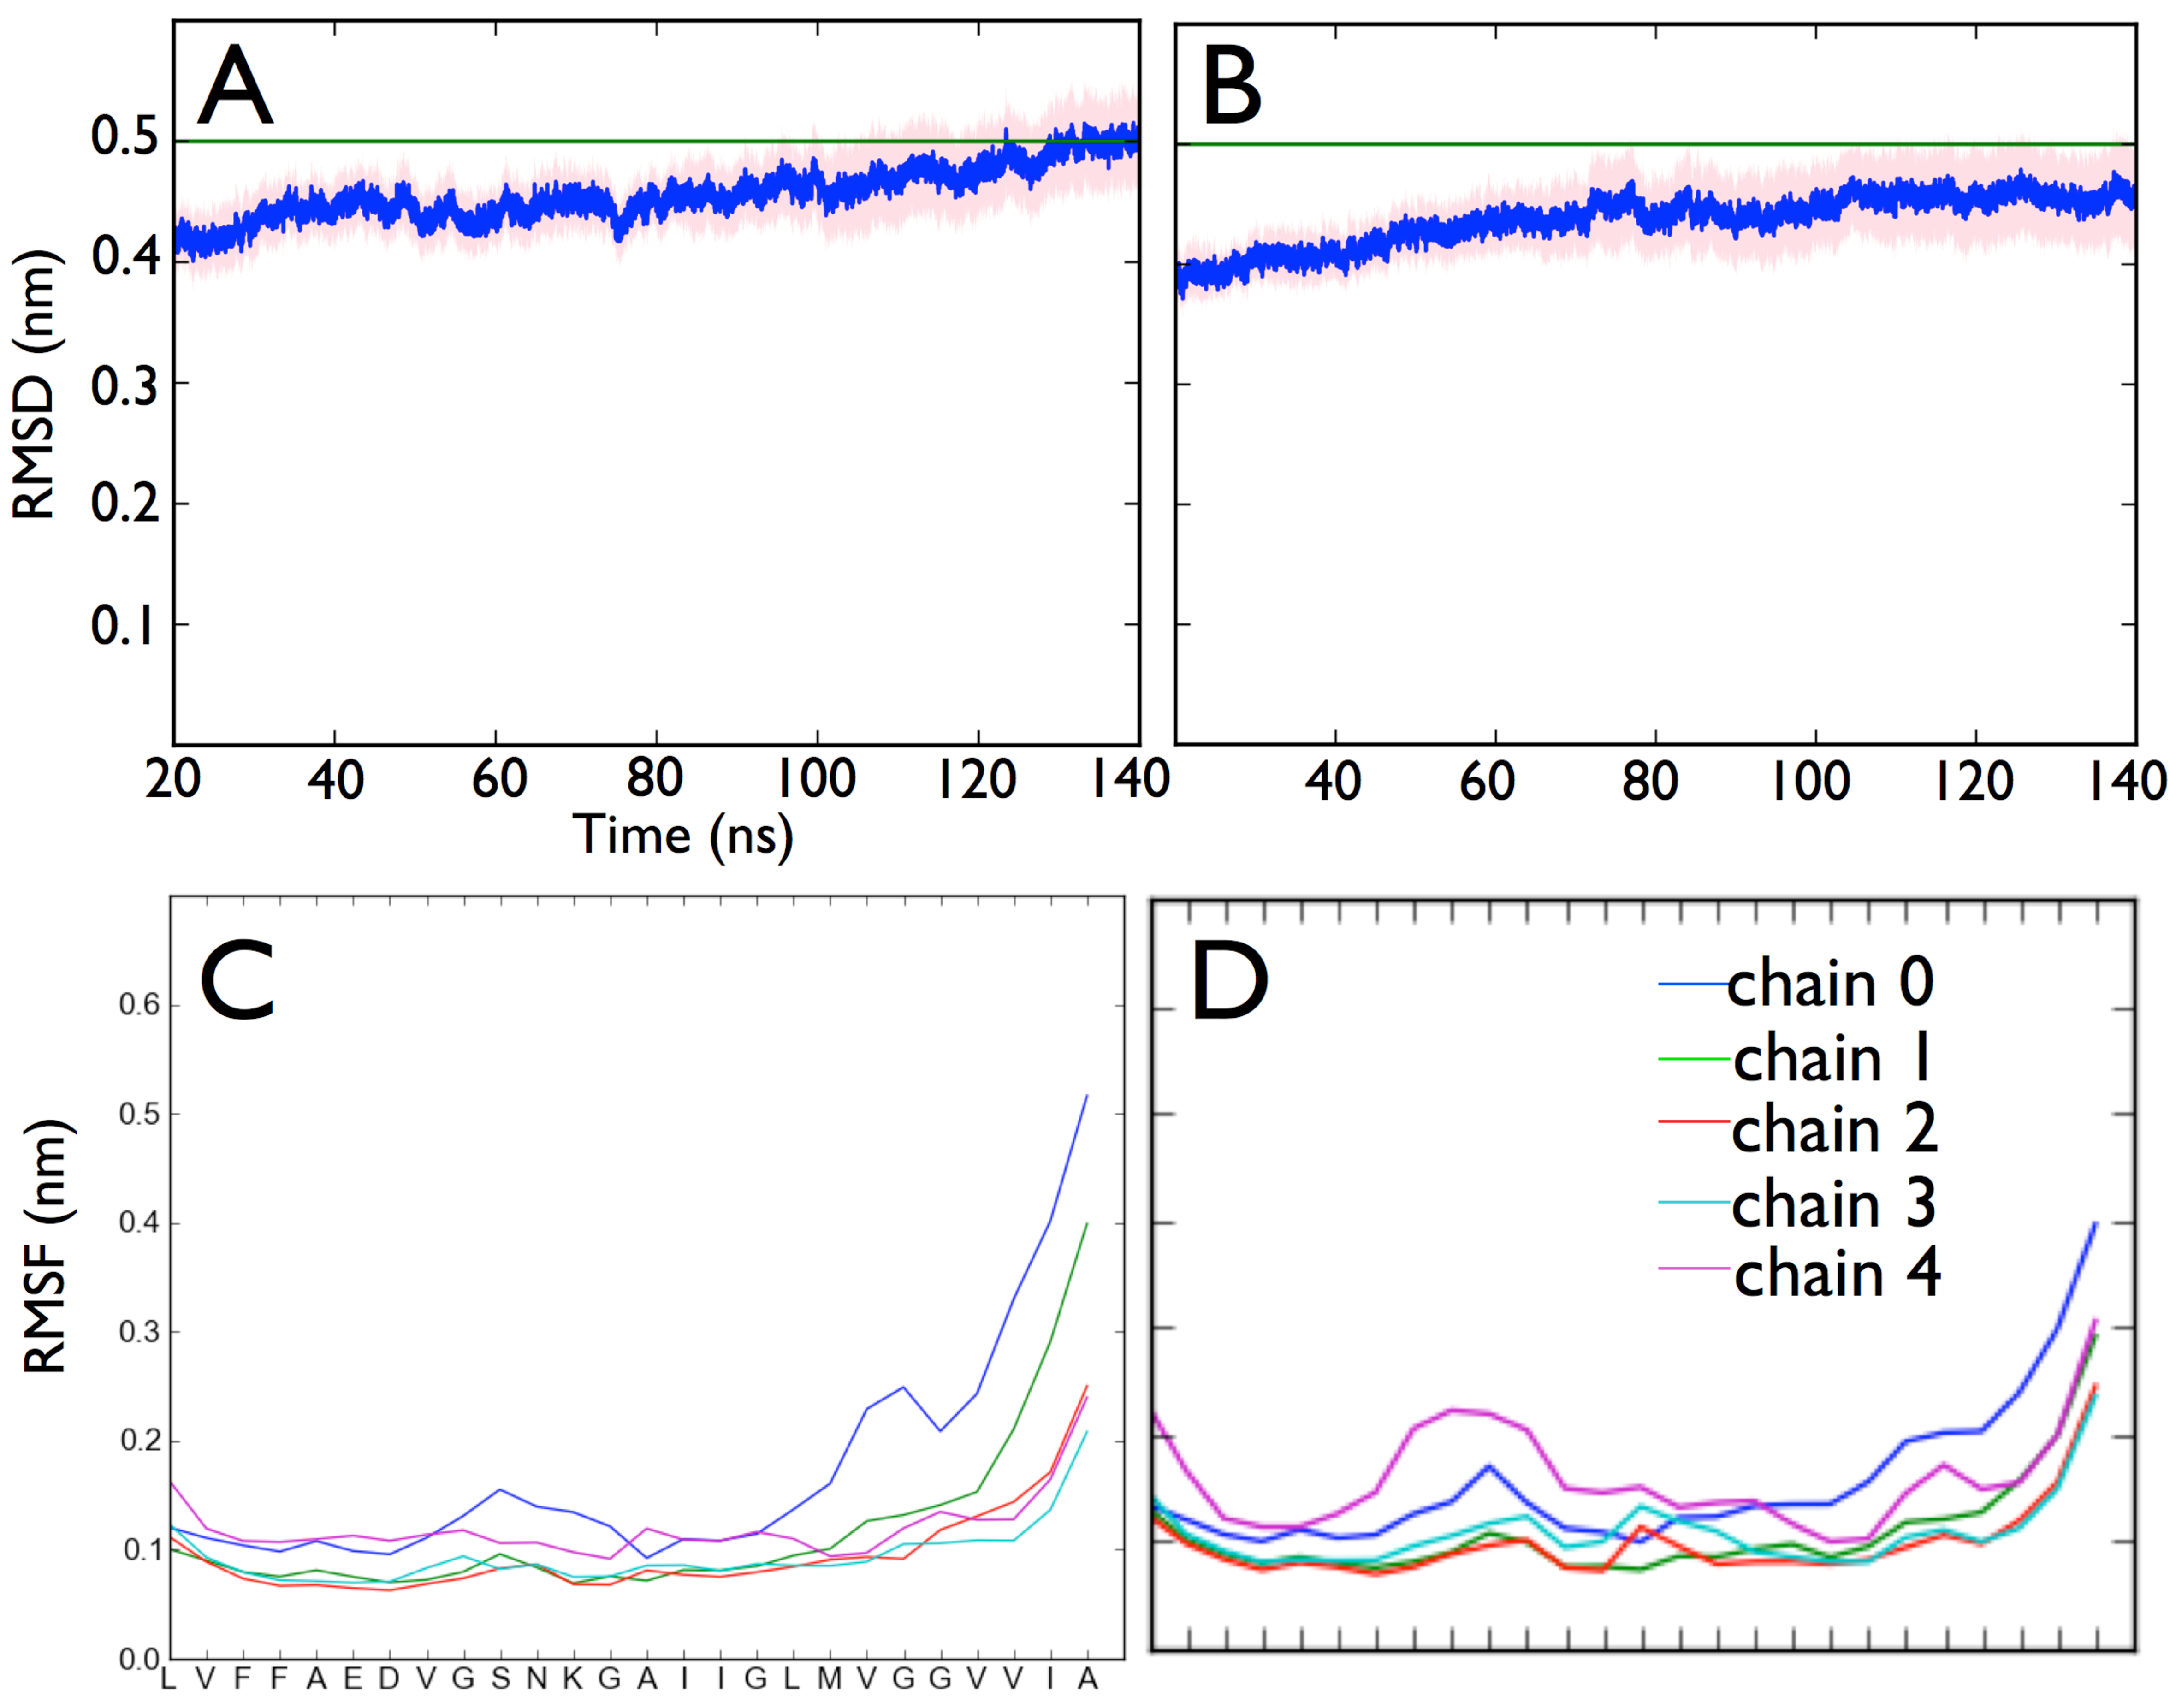
\includegraphics[width=5in]{figures/results3/protofibril_dynamics2.pdf}
% \caption[Secondary structure of protofibril]{(A) chain-chain (B) Secondary structure of fibril}
% \label{fig:protofibril_dynamics}
%\end{figure}

%\begin{figure}[htbp]
%  \centering
%  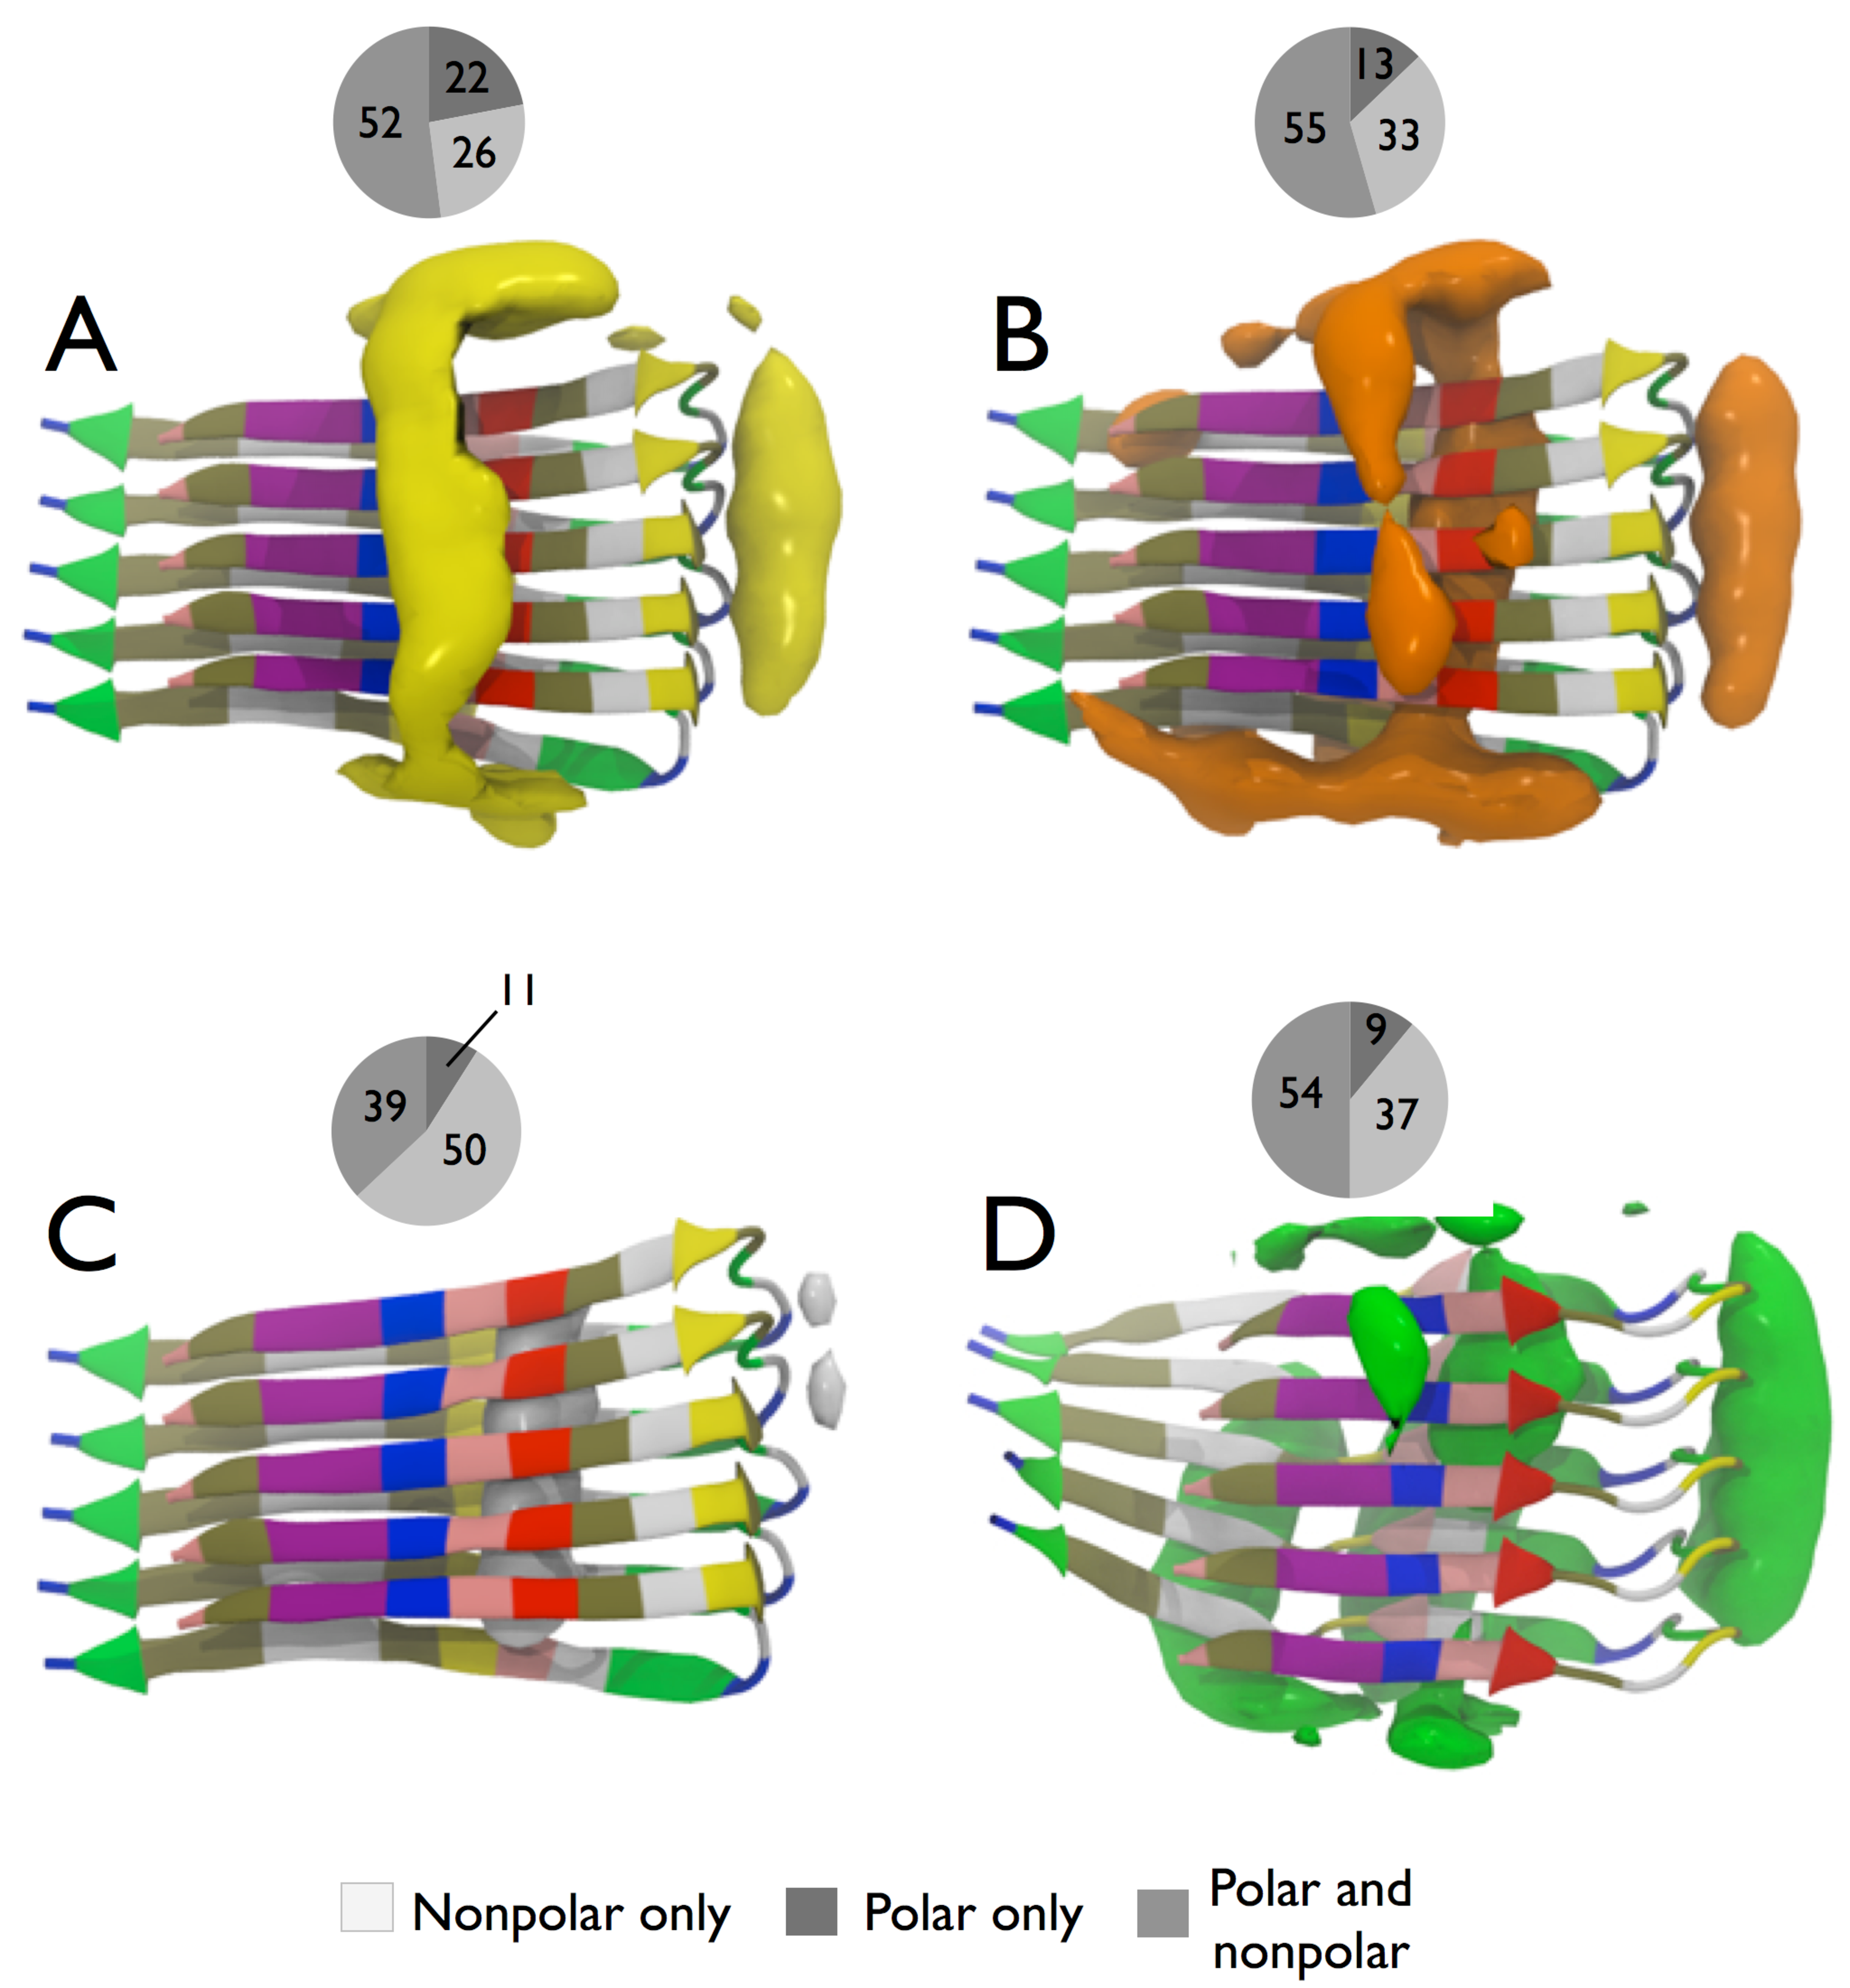
\includegraphics[width=6in]{figures/results3/binding_sdf_pie_chart.pdf}
%  \caption[Spatial probability distribution of bound solutes]{Comparisons of the spatial probability densities for (A) scyllo-inositol, (B) chiro-inositol (C) glycerol and (D) glucose.}
%  \label{fig:spatial_binding}
%\end{figure}

%\begin{figure}[htbp]
% \centering
% 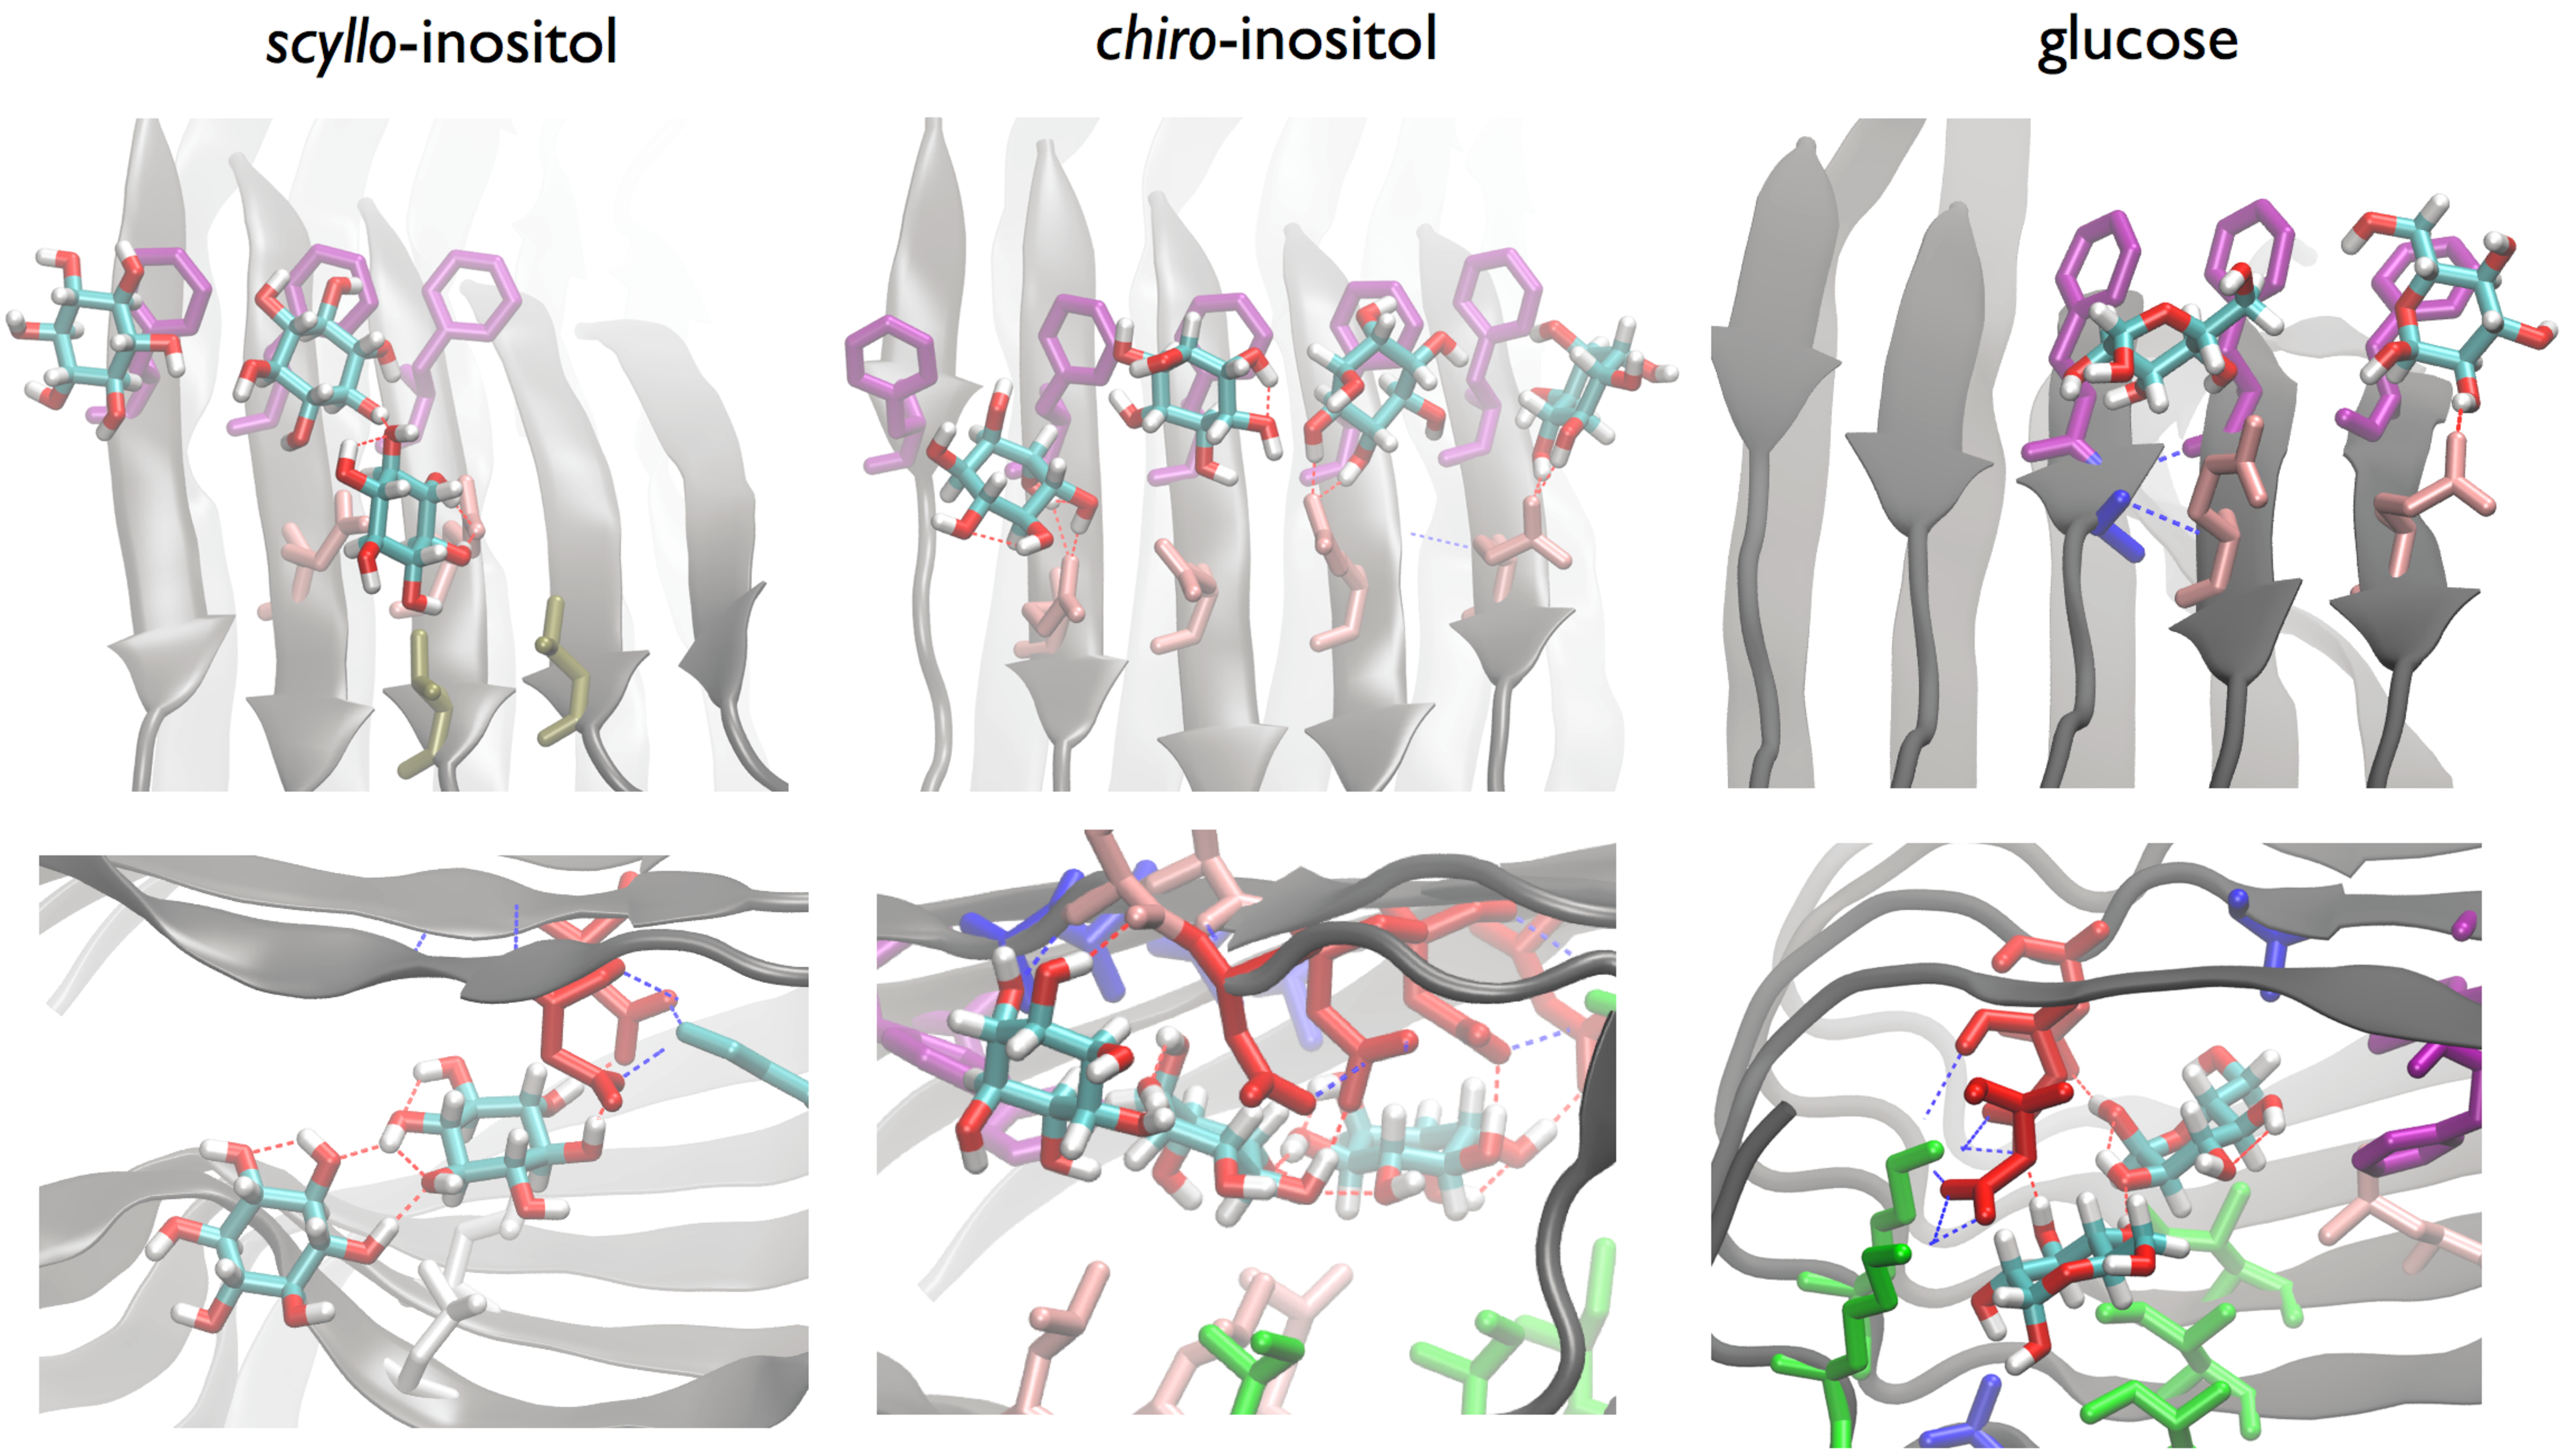
\includegraphics[width=6.5in]{figures/results3/detailed_binding_modes.pdf}
% \caption[Example binding modes of scyllo-inositol, chiro-inositol, and glucose to the protofibril]{Binding modes of scyllo-inositol, chiro-inositol and glucose to the $\beta$1 face (top row) and channel-like groove (bottom row). Residues that are within 4 \angstrom\ of a bound solute are represented in stick form. Protein is represented as a cartoon in gray.  Residues Phe, Glu, Asp, Lys and Ile are shown in colors purple, pink, red, green, and light green, respectively.}
% \label{fig:detailed_binding_modes}
%\end{figure}

%\begin{figure}[htbp]
%  \centering
%  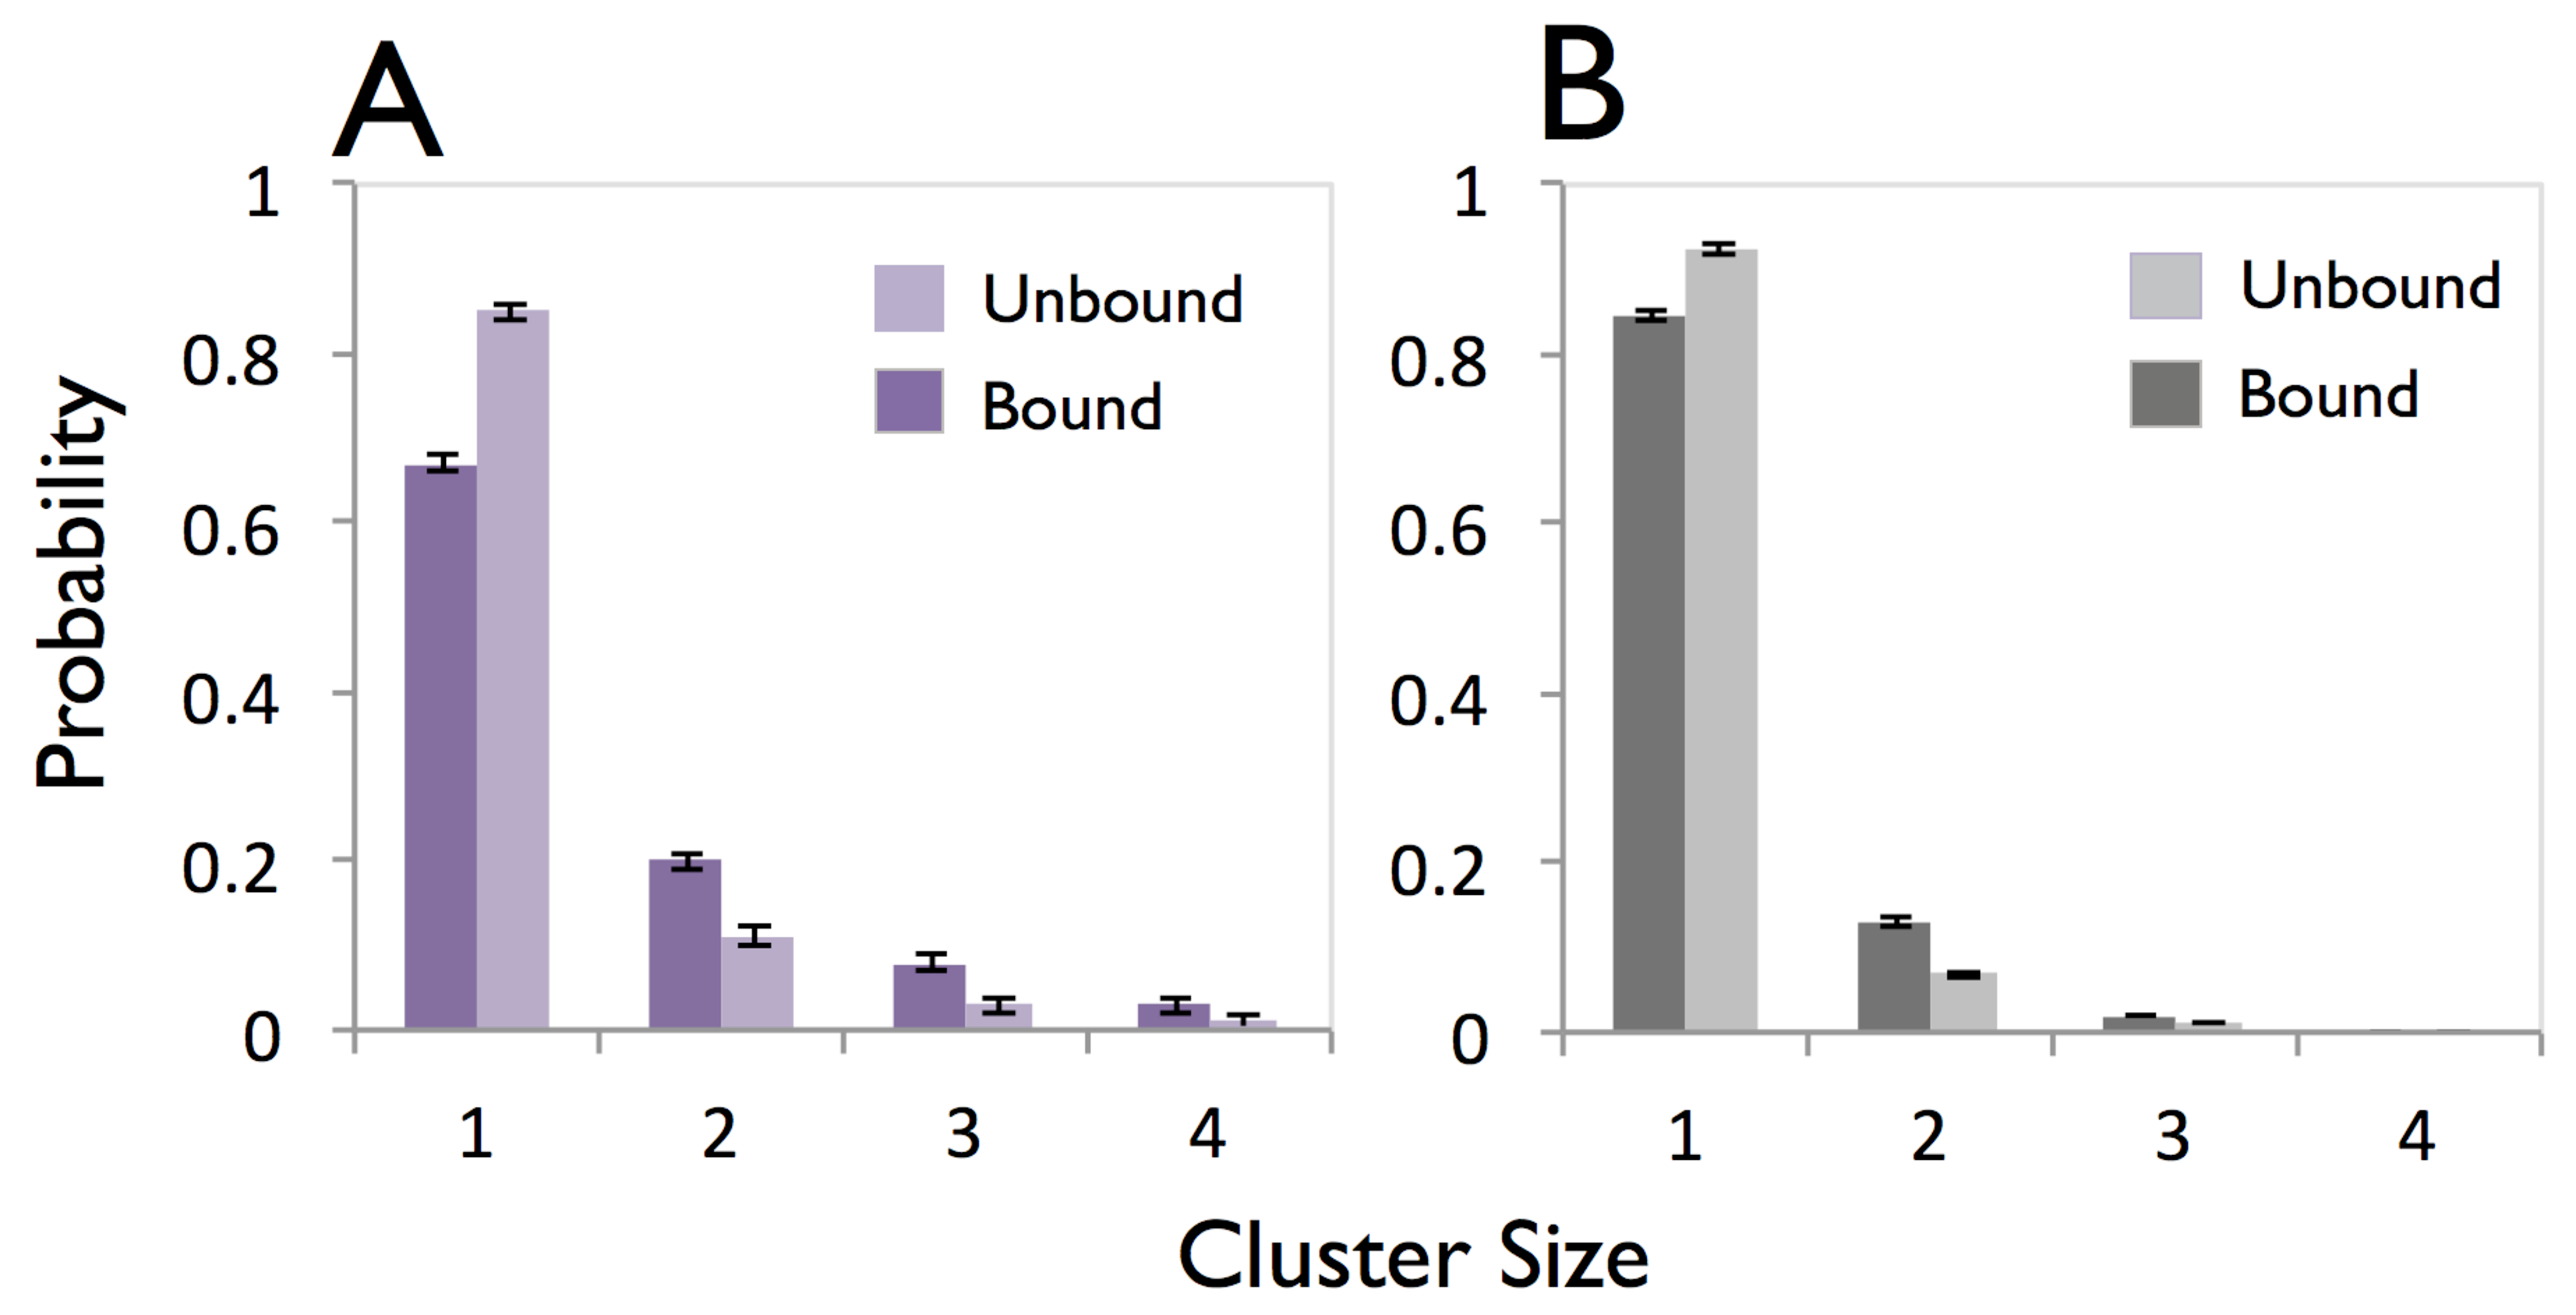
\includegraphics[width=6in]{figures/results3/clustered_binding.pdf}
%  \caption[Clustered binding of solutes at the surface of the protofibril]{Bound versus unbound cluster histograms for each solute.}
%  \label{fig:cluster_binding}
%\end{figure}

% Remove -- all of this information is already contained and is more clearly captured in the contact map
%\begin{figure}[htbp]
%  \centering
%  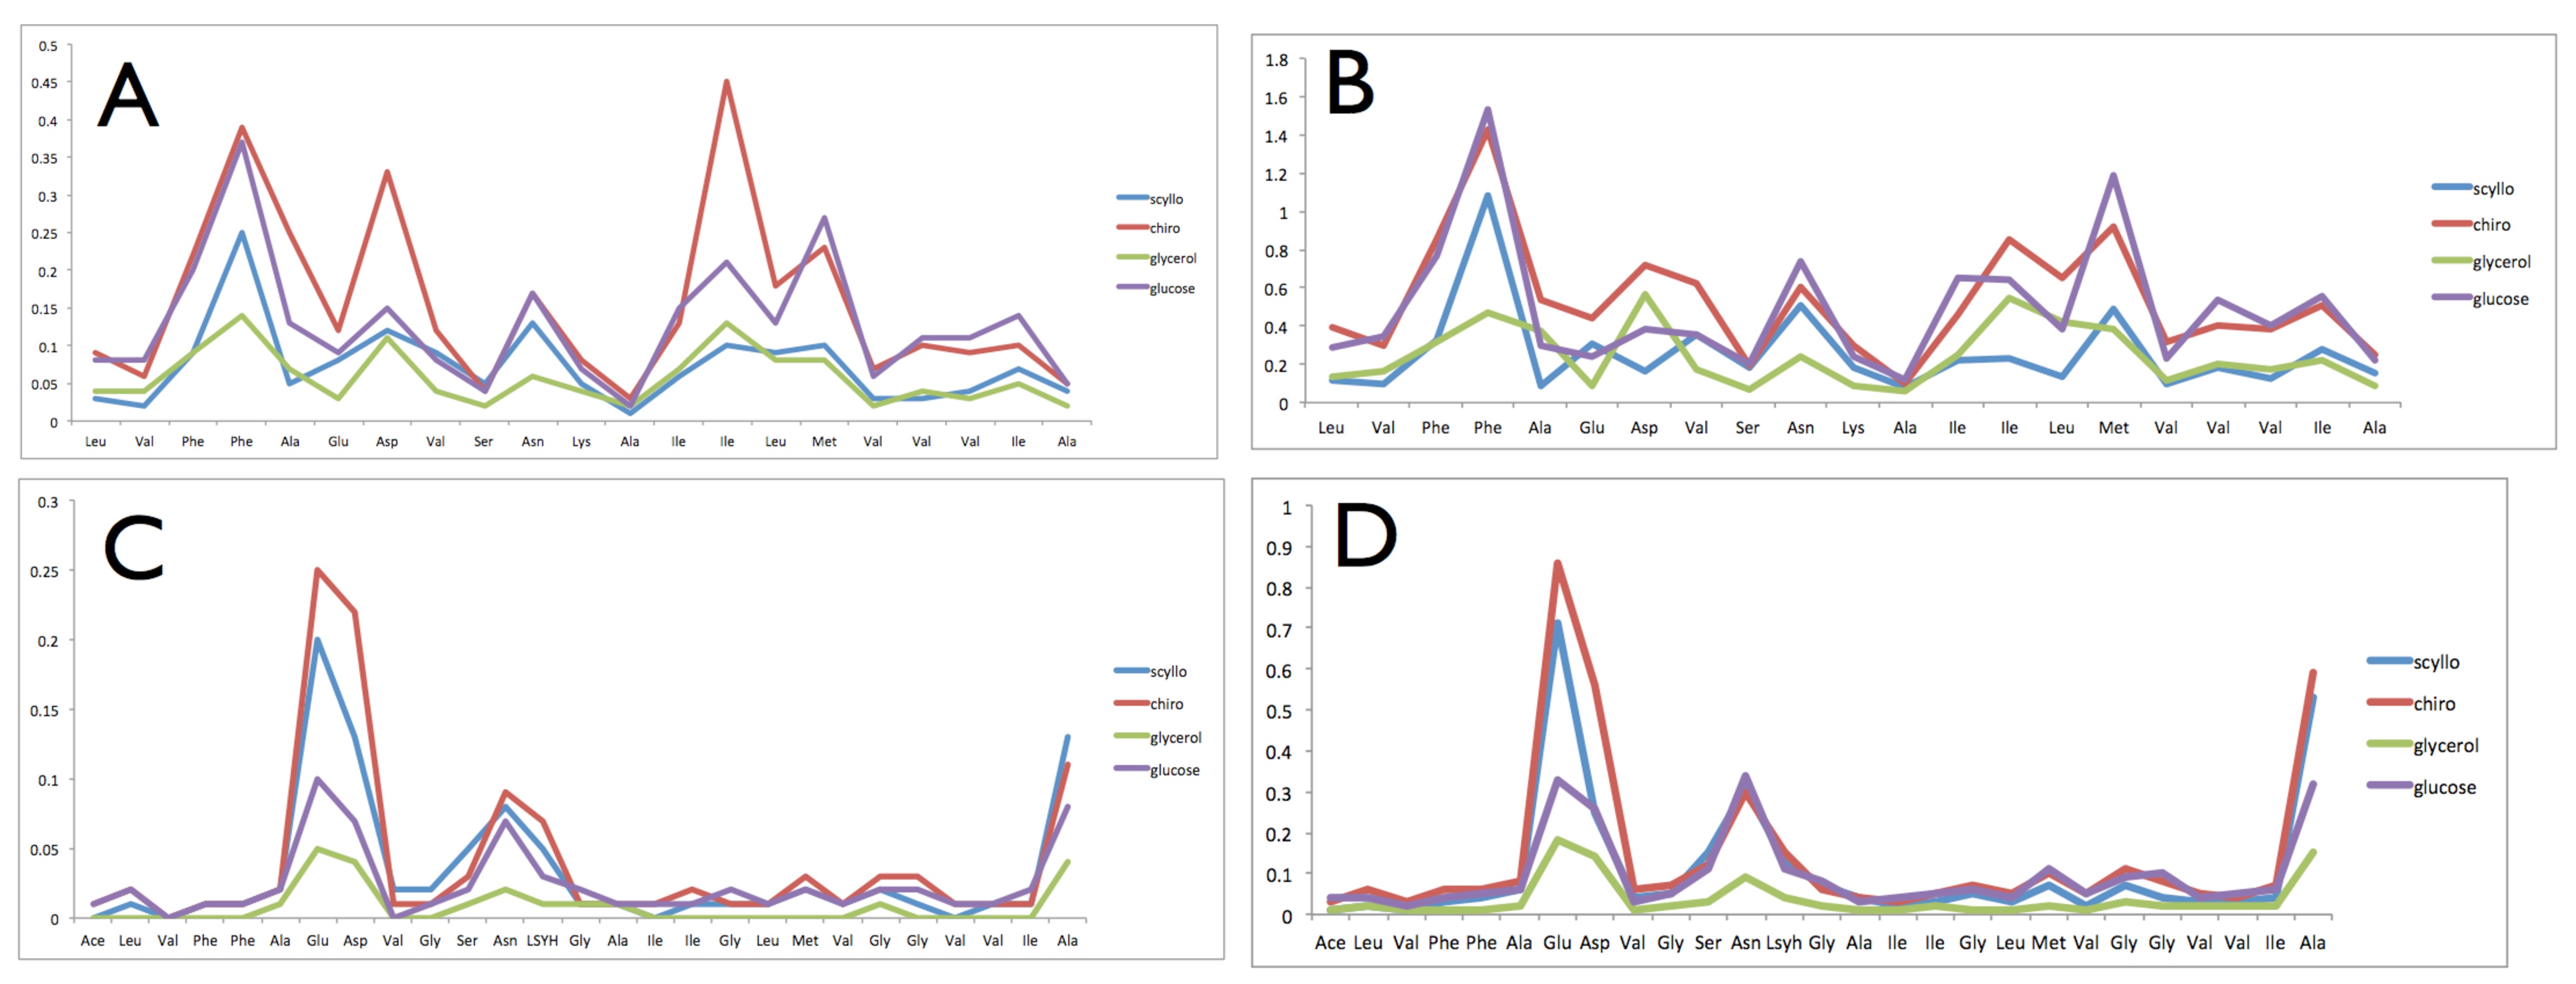
\includegraphics[width=6in]{figures/results3/binding_propensity_per_residue.pdf}
%  \caption[Binding propensity]{Binding propensity per residue of scyllo-inositol, chiro-inositol, glycerol and glucose. Nonpolar binding propensities are depicted in (A) and (B), and hydrogen bonding propensities in (C) and (D).}
%% Try to put nonpolar and hydrogen bonding for each ligand on separate panels. When put together it�s a little difficult to emphasize the differences
%  \label{fig:binding_propensity}
%\end{figure}



\begin{singlespace}
\addcontentsline{toc}{section}{Bibliography}
\bibliographystyle{elsart-num}
\bibliography{results3/results3}
\end{singlespace}

